\documentclass[11pt,a4paper]{article}
\usepackage[margin=2.3cm]{geometry}
\usepackage{amsmath,amssymb,bm}
\usepackage{siunitx}
\usepackage{booktabs}
\usepackage{nicefrac}
\usepackage{graphicx}
\usepackage{tikz}
\usetikzlibrary{arrows.meta,calc,positioning,patterns}
\usepackage{pgfplots}
\pgfplotsset{compat=1.17}
\usepackage{enumitem}
\usepackage{float}
\tikzset{capt/.style={text width=5.2cm,align=center}}
\usepackage[colorlinks=true,linkcolor=blue!60!black,urlcolor=blue!60!black]{hyperref}
\usepackage{fancyhdr}
\usepackage{tcolorbox}
\tcbuselibrary{skins,breakable}
\sisetup{per-mode=symbol,detect-all}

\newtcolorbox{keybox}[1]{title={#1},colback=blue!4,colframe=blue!50!black,fonttitle=\bfseries,breakable}
\newtcolorbox{examplebox}[1]{title={#1},colback=green!4,colframe=green!40!black,fonttitle=\bfseries,breakable}
\newtcolorbox{aerobox}[1]{title={#1},colback=orange!5,colframe=orange!60!black,fonttitle=\bfseries,breakable}

\pagestyle{fancy}
\fancyhf{}
\lhead{
\includegraphics[height=0.6cm]{logos/itu_logo_laci.pdf}\ \ UCK 364E Design of Machine Elements}
\setlength{\headheight}{20pt}
\rhead{Lecture 5 -- Notes}
\cfoot{\thepage}

\title{\textbf{UCK 364E Design of Machine Elements}\\[4pt]
\Large Lecture 5: Thread Standards and Power Screws\\[2pt]
\large Thread geometry, the aerospace profiles, and the screw as a machine}
\author{Prof.\ Dr.\ Onur Tunçer\\ Department of Aeronautical Engineering, Istanbul Technical University}
\date{Fall 2026}

\begin{document}
\maketitle

\section*{Learning objectives}
By the end of this lecture you should be able to:
\begin{enumerate}[nosep]
  \item Read and write a thread designation in both the ISO metric and the Unified systems, and say what each field means.
  \item Explain what distinguishes the UNJ and MJ aerospace profiles from UN and ISO metric, and why that difference exists.
  \item Compute the tensile stress area of a thread and use it correctly.
  \item Explain why an aerospace bolt thread is rolled after heat treatment, in the language of Lectures 2 to 4.
  \item Choose a thread engagement length from the nut material, so that the bolt breaks before the thread strips.
  \item Compute the bolt and member stiffnesses of a clamped joint, the joint constant $C$, and explain what the stress cone has to do with both.
  \item Select a preload from the proof load, convert it to a tightening torque through the nut factor, and say why that conversion is unreliable.
  \item Say what a washer is for, structurally, and which washer belongs in which application.
  \item Choose a head type for a joint, distinguish a shear head from a tension head, and say what the under-head fillet does.
  \item Specify a countersink: the included angle, the depth limit, and when the sheet must be dimpled instead.
  \item Explain why a countersunk hole is the critical fatigue detail in a lap joint, and where the crack starts.
  \item Choose a drive recess, and say what cam-out costs you.
  \item Choose a nut for a joint, distinguish a tension nut from a shear nut, and name the three
        things aerospace accepts as locking.
  \item Treat prevailing torque as a specification with two limits, and say what a self-locking
        nut may not be used for.
  \item Compute a turn-of-nut angle from the joint stiffnesses, and judge whether that method
        suits the joint in front of you.
  \item Check a power screw as a column: root diameter, end fixity, full extension, and the
        slenderness limit beyond which Euler no longer applies.
  \item Say why galling destroys a preload, which materials gall, and what to do about it.
  \item Choose a fastener material for a given structure from the two galvanic rules, and say
        why the fastener must always be the cathode.
  \item Compute the preload change a temperature excursion produces in a dissimilar-metal
        joint, and name the four things that change if the structure is a laminate.
  \item Lay out a bolt circle, and explain why the bolts are sized by spacing and preload rather than by the load they carry.
  \item Derive and apply the torque relations for a power screw, raising and lowering.
  \item Test a screw for self-locking and compute its efficiency.
  \item Size a power-screw nut against thread bearing pressure, and explain why wear, not strength, usually sets its life.
\end{enumerate}

\section{Why this lecture exists}

A helix does two quite different jobs in an aircraft, and the same geometry serves both.

The first job is \textbf{fastening}. A threaded fastener is a device for generating and holding a large
clamping force with a small tool. An airliner contains of the order of a million of them. Their design
is the subject of Lecture 6; what we need first is the language --- what a thread \emph{is}, how it is
specified, and which features of its geometry matter.

The second job is \textbf{motion}. A power screw converts rotation into translation and torque into axial
force. It appears wherever an aircraft needs a large, slow, controllable linear motion that must hold
position when the power is removed: flap and slat drives, landing-gear actuators, cargo doors, seat
and cabin mechanisms, and --- the example this lecture ends with --- the horizontal stabiliser trim
actuator.

These two jobs pull the design of the thread in opposite directions, and that tension organises
everything below.

\begin{keybox}{The same geometry, two opposite objectives}
In a \emph{fastener} you want the thread to be as efficient as possible at converting torque into
preload, and you want the thread root to be as benign as possible in fatigue, because the root is a
notch in a part that will see millions of cycles. You do \emph{not} want the screw to move.

In a \emph{power screw} you want the thread to move under load, repeatably, for thousands of cycles ---
and in most aerospace applications you also want it to \emph{stop} moving and hold its position the
instant the drive is removed. Those last two requirements are in direct conflict: a thread that slides
easily is efficient but will not hold, and a thread that holds will waste most of the input power as
friction.

Everything in this lecture is a consequence of one of these two tensions.
\end{keybox}

\begin{aerobox}{The oldest screw is a pump}
The screw as a \emph{machine} is about two thousand years older than the screw as a \emph{fastener}.
The earliest references to the water screw --- the \emph{cochlias} --- date from between
\textbf{250 and 220 BC}, and antiquity attributed it to Archimedes of Syracuse
(\textbf{287--212 BC}):

\begin{itemize}[leftmargin=*,itemsep=1pt]
\item Moschion's account of the \emph{Syracusia}, the enormous ship built for Hiero II of Syracuse,
  records that her bilge could be emptied by \emph{one man} using ``an invention of Archimedes''.
  That is the first screw known to have gone to sea, and it went as a pump.
\item Diodorus Siculus (1st century BC) describes it irrigating the Nile delta and draining the
  Roman silver mines in Spain, where he calls it the ``Egyptian screw''.
\item Vitruvius, \emph{De architectura} X.6 (written 27--22 BC), gives the earliest surviving
  \emph{construction} account: how to set out the spiral on a round beam, how many starts to use
  (he specifies eight), and at what inclination to mount it.
\end{itemize}

\medskip
The attribution is disputed, and the dispute is worth knowing. Stephanie Dalley has argued that an
inscription of the Assyrian king Sennacherib describes bronze water screws irrigating the gardens at
Nineveh --- centuries before Archimedes --- and J.\,P.\ Oleson has pointed out that no ancient
source ever explains \emph{why} the device came to carry Archimedes' name. Engineering history is
like this more often than textbooks admit.
\end{aerobox}

\begin{keybox}{Why Archimedes belongs in a lecture on screws}
Because his machine is \textbf{the same geometry doing the other job}, and it makes the organising
idea of this lecture concrete.

\medskip
Wrap an inclined plane around a cylinder and you have a helix. Now turn it. Something has to move
along the axis --- and what moves depends only on what you hold still:

\begin{center}\footnotesize
\begin{tabular}{@{}p{3.6cm}p{1.9cm}p{8.0cm}@{}}
\toprule
Hold still & Turn & What you get\\
\midrule
the nut & the screw & a \textbf{power screw}: the nut translates, torque becomes axial force\\[2pt]
nothing --- an open flight & the screw & an \textbf{Archimedes screw}: the \emph{material} translates\\[2pt]
the nut, with a tiny lead & the screw & a \textbf{bolt}: motion so slow it cannot back-drive\\
\bottomrule
\end{tabular}
\end{center}

\medskip
Every relation in \S\ref{sec:helix} --- lead $L=np$, the helix angle $\tan\lambda = L/\pi d_m$, the
number of starts --- applies unchanged to all three. Only the \emph{useful output} differs: axial
transport, axial force, or clamping force that must never move. Vitruvius' eight-start screw is a
multi-start thread chosen, exactly as you would choose one today, for lead per turn.
\end{keybox}

\begin{figure}[H]\centering
\resizebox{0.92\textwidth}{!}{% The Archimedes screw: the same helix, carrying material instead of clamping.
\begin{tikzpicture}[>=Latex,line join=round]
\tikzset{
  water/.style={fill=cyan!35,draw=cyan!60!black,thin},
  tube/.style={draw=black!60,thick},
  flight/.style={draw=blue!55!black,thick},
  lb/.style={font=\small},
  sm/.style={font=\scriptsize,text=black!65}
}
\def\ang{27}      % inclination
\def\r{0.72}      % tube radius
\def\p{1.55}      % pitch (projected)
\def\Lx{9.3}      % length along the axis

% ---------- lower reservoir ----------
\fill[cyan!22,draw=cyan!55!black] (-2.90,-1.95) rectangle (1.40,-0.05);
\draw[black!55,thick] (-2.90,-2.10) -- (-2.90,-0.05) (1.40,-2.10) -- (1.40,-0.05);
\draw[black!55,thick] (-3.00,-2.10) -- (1.50,-2.10);
\node[sm,anchor=north] at (-1.0,-2.18) {source};

\begin{scope}[rotate=\ang]

% ---------- tube ----------
\draw[tube,fill=black!3] (0,-\r) rectangle (\Lx,\r);

% ---------- water pockets, one per pitch, lying on the low side ----------
\foreach \i in {0,1,...,5}{
  \pgfmathsetmacro\xc{0.72+\i*\p}
  \fill[water] (\xc-0.52,-\r+0.02) -- (\xc+0.52,-\r+0.02)
     -- (\xc+0.40,-\r+0.40) -- (\xc-0.40,-\r+0.40) -- cycle;
}

% ---------- the flight: near edge solid, far edge dashed ----------
\draw[flight,domain=0:\Lx,samples=400,variable=\x]
  plot ({\x},{\r*sin(360*\x/\p)});
\draw[flight,dashed,opacity=0.55,domain=0:\Lx,samples=400,variable=\x]
  plot ({\x},{-\r*sin(360*\x/\p)});

% ---------- pitch dimension ----------
\draw[<->,gray!80!black,thin] (0.385,\r+0.34) -- (0.385+\p,\r+0.34);
\node[font=\small,fill=white,inner sep=1pt] at (0.385+\p/2,\r+0.34) {$p$};

% ---------- rotation ----------
\draw[->,red!65!black,very thick] ({\Lx-2.0},{\r+1.30}) arc (-70:200:0.40);
\node[font=\small,text=red!65!black,anchor=west] at ({\Lx-1.45},{\r+1.30}) {turn};

% ---------- outlet ----------
\draw[tube] (\Lx,\r) -- (\Lx+0.55,\r) (\Lx,-\r) -- (\Lx+0.55,-\r);
\end{scope}

% ---------- discharge ----------
\coordinate (out) at ({(\Lx+0.55)*cos(\ang)-(-\r)*sin(\ang)},{(\Lx+0.55)*sin(\ang)+(-\r)*cos(\ang)});
\draw[water,line width=1.4pt,draw=cyan!60!black] (out) .. controls +(0.35,-0.45) and +(0,0.55) .. ($(out)+(0.6,-1.5)$);
\node[sm,anchor=north west,align=left] at ($(out)+(0.42,-1.55)$) {delivered\\ uphill};

% ---------- the idea, stated ----------
\node[lb,anchor=north west,align=left,text width=7.4cm] at (-3.0,-2.75)
 {\textbf{The same helix, the other job.} Hold the nut still and the \emph{nut} travels: a power
  screw. Leave the flight open and the \emph{material} travels: a pump. Turn it so slowly it cannot
  back-drive, and it is a bolt.};
\node[sm,anchor=north west,align=left,text width=7.0cm] at (-3.0,-4.95)
 {$L=np$ and $\tan\lambda = L/\pi d_m$ hold for all three. Vitruvius specified \emph{eight} starts
  --- a multi-start thread, chosen for lead per turn, exactly as you would choose one today.};

\end{tikzpicture}
}
\caption{The Archimedes screw. The flight is open, so the water --- not a nut --- is what travels
along the axis. Every geometric relation in \S\ref{sec:helix} applies to it unchanged.}
\label{fig:archimedes}
\end{figure}

\medskip
The machine is still working. Archimedes screws lift sewage in treatment plants because they are
indifferent to solids and to varying flow; they drained the Dutch polders through the Golden Age;
and since the 1990s they have been run \emph{backwards}, as low-head hydro turbines, over flows of
\SIrange{0.01}{14.5}{m^3/s} and heads of \SIrange{0.1}{10}{m}. A screw run backwards by its load is
a machine that is not self-locking --- which is the subject of \S\ref{sec:selflock}, and the reason
a jackscrew in a stabiliser is designed so that it can never happen.

\section{Thread geometry and terminology}

\subsection{Pitch, lead and starts}

The \textbf{pitch} $p$ is the axial distance between corresponding points on adjacent threads. The
\textbf{lead} $L$ is the axial distance the nut advances in one turn of the screw. For a single-start
thread they are equal. For an $n$-start thread,
\[
\boxed{\,L = n\,p\,}
\]
Multiple starts buy speed at the expense of self-locking, as we shall see; they are common in cheap
mechanisms and rare in flight-critical ones.

\begin{figure}[H]\centering
\resizebox{0.56\textwidth}{!}{
\begin{tikzpicture}[scale=0.95,>=Stealth,font=\scriptsize,line join=round]
\def\hh{0.78}
% ---------------- single start ----------------
\begin{scope}
\foreach \x in {0,1.4,2.8,4.2}{
  \fill[blue!55!black] (\x-0.17,0) -- (\x,\hh) -- (\x+0.17,0) -- cycle;
  \draw[thick] (\x-0.17,0) -- (\x,\hh) -- (\x+0.17,0);}
\draw[thick] (-0.55,0) -- (4.95,0); \draw[thick] (-0.55,-0.45) -- (4.95,-0.45);
\fill[gray!18] (-0.55,-0.45) rectangle (4.95,0);
\draw[<->] (0,\hh+0.30) -- (1.4,\hh+0.30) node[midway,above,font=\tiny]{$p$};
\draw[<->,blue!55!black,thick] (0,\hh+0.90) -- (1.4,\hh+0.90)
  node[midway,above,font=\tiny,black]{$L=p$};
\node[anchor=north,font=\bfseries] at (2.2,-0.62) {single start};
\node[anchor=north,align=center,font=\tiny,text width=4.6cm] at (2.2,-0.92)
  {one continuous thread; the nut advances one pitch per turn};
\end{scope}
% ---------------- double start ----------------
\begin{scope}[yshift=-3.5cm]
\foreach \x in {0,1.4,2.8,4.2}{
  \fill[blue!55!black] (\x-0.17,0) -- (\x,\hh) -- (\x+0.17,0) -- cycle;
  \draw[thick] (\x-0.17,0) -- (\x,\hh) -- (\x+0.17,0);}
\foreach \x in {0.7,2.1,3.5}{
  \fill[orange!75!black] (\x-0.17,0) -- (\x,\hh) -- (\x+0.17,0) -- cycle;
  \draw[thick] (\x-0.17,0) -- (\x,\hh) -- (\x+0.17,0);}
\draw[thick] (-0.55,0) -- (4.95,0); \draw[thick] (-0.55,-0.45) -- (4.95,-0.45);
\fill[gray!18] (-0.55,-0.45) rectangle (4.95,0);
\draw[<->] (0,\hh+0.30) -- (0.7,\hh+0.30) node[midway,above,font=\tiny]{$p$};
\draw[<->,blue!55!black,thick] (0,\hh+0.90) -- (1.4,\hh+0.90)
  node[midway,above,font=\tiny,black]{$L=2p$};
\node[anchor=north,font=\bfseries] at (2.2,-0.62) {double start};
\node[anchor=north,align=center,font=\tiny,text width=5.4cm] at (2.2,-0.92)
  {\emph{two} separate threads interleaved. The pitch is unchanged ---
   but one turn now advances the nut by two pitches};
\end{scope}
\end{tikzpicture}
}
\caption{Pitch is a property of the thread form and does not change. Lead is how far the nut travels
per turn. A second start doubles $L$ with $p$ untouched --- so $\tan\lambda$ doubles, and a screw that
was comfortably self-locking may stop being so.}
\end{figure}

\subsection{Diameters and the basic profile}

Three diameters matter, and they are not interchangeable:
\begin{itemize}[nosep]
  \item the \textbf{major diameter} $d$, measured at the crests of an external thread --- the nominal size;
  \item the \textbf{minor diameter} $d_3$ (or $d_r$), measured at the roots --- this is where the section is smallest, and where the thread will break;
  \item the \textbf{pitch diameter} $d_2$, the diameter of the imaginary cylinder on which the thread and the groove are equally wide. This is the diameter that actually controls fit, and it is what a thread gauge measures.
\end{itemize}

Both ISO metric (\textbf{ISO 68-1}) and Unified (\textbf{ASME B1.1}) threads are built on the same
\SI{60}{\degree} triangular basic profile, truncated at crest and root.

\begin{figure}[H]\centering

\begin{tikzpicture}[scale=1.25,>=Stealth,font=\scriptsize,line join=round]
\def\hh{1.083}
\fill[gray!14]
  (-0.25,0) -- (0.25,0) -- (0.875,\hh) -- (1.125,\hh) -- (1.75,0) -- (2.25,0)
  -- (2.875,\hh) -- (3.125,\hh) -- (3.75,0) -- (4.25,0) -- (4.875,\hh) -- (5.125,\hh)
  -- (5.75,0) -- (6.1,0) -- (6.1,-0.75) -- (-0.25,-0.75) -- cycle;
\draw[thick]
  (-0.25,0) -- (0.25,0) -- (0.875,\hh) -- (1.125,\hh) -- (1.75,0) -- (2.25,0)
  -- (2.875,\hh) -- (3.125,\hh) -- (3.75,0) -- (4.25,0) -- (4.875,\hh) -- (5.125,\hh)
  -- (5.75,0) -- (6.1,0);
\draw[thick] (-0.25,-0.75) -- (6.1,-0.75);
\draw[blue!55!black,dashed] (-0.55,\hh) -- (6.3,\hh) node[right,black]{crest / major $d$};
\draw[blue!55!black,dashed] (-0.55,0.433) -- (6.3,0.433) node[right,black]{pitch $d_2$};
\draw[blue!55!black,dashed] (-0.55,0) -- (6.3,0) node[right,black]{root / minor $d_3$};
\draw[<->] (1.0,\hh+0.95) -- (3.0,\hh+0.95) node[midway,above]{pitch $p$};
\draw[gray!60,line width=0.3pt] (1.0,\hh) -- (1.0,\hh+0.99);
\draw[gray!60,line width=0.3pt] (3.0,\hh) -- (3.0,\hh+0.99);
% included thread angle: extend the two flanks of one tooth to the sharp-V apex
\draw[red!70!black,line width=0.5pt] (2.25,0) -- (3.0,1.300);
\draw[red!70!black,line width=0.5pt] (3.75,0) -- (3.0,1.300);
\draw[red!70!black] ($(3.0,1.300)+(255.4:0.34)$) arc (255.4:284.6:0.34);
\draw[->,red!70!black,line width=0.4pt] (3.95,1.62) -- (3.18,1.18);
\node[red!70!black,anchor=west,align=left,font=\tiny] at (3.97,1.62)
  {$2\alpha=60^\circ$\\ at the sharp-V apex};
\draw[<->] (5.95,0) -- (5.95,\hh) node[midway,left,font=\tiny]{$h$};
\draw[dash pattern=on 6pt off 2pt on 1pt off 2pt] (-0.55,-1.05) -- (6.3,-1.05);
\node[anchor=west] at (6.3,-1.05) {screw axis};
\end{tikzpicture}

\caption{The \SI{60}{\degree} basic profile common to ISO metric and Unified threads, shown as an axial
section of an external thread. The flanks are the load-carrying surfaces; the root is the fatigue-critical
feature.}
\end{figure}

\subsection{The helix angle}\label{sec:helix}

Unwrap one turn of the helix at the mean diameter $d_m \approx d_2$ and it becomes a right triangle of
base $\pi d_m$ and height $L$. The \textbf{lead angle} $\lambda$ follows:
\[
\boxed{\,\tan\lambda = \frac{L}{\pi d_m}\,}
\]
This single relation governs the whole of the power-screw analysis. A fastener thread has a small
$\lambda$ --- typically \SIrange{2}{4}{\degree} --- which is why it is efficient at holding and hopeless
at moving.

\section{Thread standards and designations}

\subsection{The two systems}

\begin{center}\small
\begin{tabular}{@{}lll@{}}
\toprule
 & \textbf{ISO metric} & \textbf{Unified (inch)}\\
\midrule
Basic profile & ISO 68-1 & ASME B1.1\\
Tolerances & ISO 965 & ASME B1.1\\
Size given by & nominal $d$ in mm & nominal $d$ in inches\\
Thread given by & pitch $p$ in mm & threads per inch $n$\\
Coarse / fine & M10$\times$1.5 / M10$\times$1.25 & UNC / UNF / UNEF\\
Designation & \texttt{M10$\times$1.5--6g} & \texttt{1/4--28 UNF--3A}\\
\bottomrule
\end{tabular}
\end{center}

\medskip
Read \texttt{M10$\times$1.5--6g}: metric thread, nominal diameter \SI{10}{mm}, pitch \SI{1.5}{mm},
tolerance class 6g (external). Read \texttt{1/4--28 UNF--3A}: nominal \SI{0.25}{in}, 28 threads per
inch, Unified Fine series, class 3A (external, close fit).

\subsection{Classes of fit}

In the Unified system, classes 1A/1B, 2A/2B and 3A/3B run from loose to close, with A external and
B internal. Class 2A/2B is general commercial practice; \textbf{3A/3B} is the close fit used where the
thread must be accurately located and consistently stressed, and it is standard for aerospace
fasteners. In ISO, the equivalents are written as a pitch-diameter tolerance followed by a
crest-diameter tolerance, as in 6g (external, general) or 4h6h (close).

\medskip
A looser class means more clearance on the pitch diameter, which means the load is shared less evenly
between engaged threads, which means the first engaged thread carries more. That is a fatigue
argument, not a convenience argument, and it is why the aerospace world pays for 3A.

\subsection{Which document governs what}

A thread callout is not finished until you have specified three separate things --- the
\textbf{profile}, the \textbf{class of fit} and the \textbf{part standard}. Leave any one of them out
and the shop is entitled to choose it for you.

\begin{center}\small
\begin{tabular}{@{}lll@{}}
\toprule
\textbf{What you must specify} & \textbf{ISO} & \textbf{Inch}\\
\midrule
Basic profile & ISO 68-1 & ASME B1.1\\
Tolerance class & ISO 965 & ASME B1.1\\
Aerospace profile & ISO 5855 (MJ) & SAE AS8879 (UNJ)\\
Material / property class & ISO 898-1 & SAE J429, AMS specifications\\
Gauging and inspection & ISO 1502 & ASME B1.2\\
The part itself & --- & AN / MS / NAS / NASM\\
\bottomrule
\end{tabular}
\end{center}

\medskip
Turkey adopts the ISO and EN documents essentially unchanged, under \textbf{TS ISO} and \textbf{TS EN
ISO} designations --- \textbf{TS EN ISO 898-1} is the property-class standard you will meet most
often. Confirm the current TS number from the TSE catalogue; adopted standards are periodically
re-issued.

\subsection{What a dimensional standard actually contains}

Everything in the tables below follows from the pitch and the basic profile. That is what a
dimensional standard is: not a catalogue, but one geometry plus the tolerance bands that let parts
made in different factories fit each other.

\begin{center}\footnotesize
\textbf{Metric coarse series} --- ISO 261 / ISO 965-1\\[3pt]
\begin{tabular}{@{}lcccccc@{}}
\toprule
Designation & $d$ & $p$ & $d_2$ & $D_1$ & $d_3$ & $A_t$\\
 & \multicolumn{5}{c}{mm} & mm$^2$\\
\midrule
M3$\times$0.5 & 3 & 0.5 & 2.675 & 2.459 & 2.387 & 5.0\\
M4$\times$0.7 & 4 & 0.7 & 3.545 & 3.242 & 3.141 & 8.8\\
M5$\times$0.8 & 5 & 0.8 & 4.480 & 4.134 & 4.019 & 14.2\\
M6$\times$1 & 6 & 1.0 & 5.350 & 4.917 & 4.773 & 20.1\\
M8$\times$1.25 & 8 & 1.25 & 7.188 & 6.647 & 6.466 & 36.6\\
M10$\times$1.5 & 10 & 1.5 & 9.026 & 8.376 & 8.160 & 58.0\\
M12$\times$1.75 & 12 & 1.75 & 10.863 & 10.106 & 9.853 & 84.3\\
\bottomrule
\end{tabular}

\smallskip
{\scriptsize $d_2=d-0.649519p$ (pitch) \quad $D_1=d-1.082532p$ (internal minor; tap-drill basis)
\quad $d_3=d-1.226869p$ (external minor at the root)}
\end{center}

\begin{center}\footnotesize
\textbf{Unified inch series} --- ASME B1.1\\[3pt]
\begin{tabular}{@{}lccccccc@{}}
\toprule
Designation & $n$ & \multicolumn{2}{c}{$d$} & $p$ & $d_2$ & $D_1$ & $A_t$\\
 & tpi & in & mm & mm & mm & mm & mm$^2$\\
\midrule
10--32 UNF & 32 & 0.1900 & 4.826 & 0.794 & 4.310 & 3.967 & 12.90\\
1/4--20 UNC & 20 & 0.2500 & 6.350 & 1.270 & 5.525 & 4.975 & 20.53\\
1/4--28 UNF & 28 & 0.2500 & 6.350 & 0.907 & 5.761 & 5.368 & 23.47\\
5/16--24 UNF & 24 & 0.3125 & 7.938 & 1.058 & 7.250 & 6.792 & 37.46\\
3/8--24 UNF & 24 & 0.3750 & 9.525 & 1.058 & 8.838 & 8.379 & 56.66\\
\bottomrule
\end{tabular}

\smallskip
{\scriptsize Same basic profile, same formulae --- but the thread is indexed by \emph{threads per
inch}, so $p=25.4/n$ is never a round number in millimetres.}
\end{center}

\begin{aerobox}{Where the two systems bite: the look-alikes}
The geometry is identical; only the unit the thread is indexed by differs. That is enough to make
them silently incompatible.

\begin{center}\small
\begin{tabular}{@{}llcc@{}}
\toprule
Inch & Metric & $\Delta d$ (\si{mm}) & $\Delta p$ (\si{mm})\\
\midrule
5/16--24 UNF & M8$\times$1 & \textbf{0.062} & \textbf{0.058}\\
10--32 UNF & M5$\times$0.8 & 0.174 & \textbf{0.006}\\
1/4--28 UNF & M6$\times$1 & 0.350 & 0.093\\
3/8--24 UNF & M10$\times$1.25 & 0.475 & 0.192\\
\bottomrule
\end{tabular}
\end{center}

\medskip
A 5/16--24 bolt and an M8$\times$1 hole differ by \SI{62}{\micro\metre} on diameter and
\SI{58}{\micro\metre} on pitch. It will start, it will feel right, and it will take torque --- then it
will strip, or hold at a fraction of its rated preload.

\medskip
This is a Turkish aerospace problem specifically. Design and manufacture here run in metric to
TS\,/\,EN\,ISO, while much of the airframe hardware on US-origin aircraft is inch to AN\,/\,MS\,/\,NAS,
and both are in the same hangar. Segregate the stock, mark the drawings, and never judge a thread by
feel.
\end{aerobox}

\subsection{Property classes}

ISO 898-1 encodes two strengths in one pair of numbers: the first number $\times100$ is the nominal
tensile strength $R_m$ in \si{MPa}, and the first $\times$ second $\times10$ is the nominal yield
strength $R_e$.

\begin{center}\small
\begin{tabular}{@{}lccl@{}}
\toprule
Class & $R_m$ (\si{MPa}) & $R_e$ (\si{MPa}) & \\
\midrule
8.8 & 800 & 640 & general structural\\
10.9 & 1000 & 900 & high strength\\
12.9 & 1200 & 1080 & highest standard class\\
\bottomrule
\end{tabular}
\end{center}

\begin{keybox}{A stronger bolt is not a free upgrade}
Steels heat-treated much above \SI{1000}{MPa} become susceptible to \textbf{hydrogen embrittlement}
and to stress-corrosion cracking. They must be baked after plating to drive the hydrogen out, and that
bake is a process requirement which does not show up on the finished part. Specifying a higher class
therefore buys you strength and a new process control to get wrong.
\end{keybox}

\subsection{Coarse or fine?}

\begin{center}\small
\begin{tabular}{@{}p{6.4cm}p{6.4cm}@{}}
\toprule
\textbf{Fine} (UNF / UNJF) & \textbf{Coarse} (UNC / metric coarse)\\
\midrule
about \SI{10}{\percent} larger $A_t$ for the same nominal size
  & deeper thread, so more strip area in a soft nut material\\[3pt]
smaller lead angle, so it resists loosening better
  & far more tolerant of damage, corrosion and plating build-up\\[3pt]
finer adjustment per turn & faster to assemble, less prone to cross-threading\\[3pt]
shallower thread, easier to damage & coarser adjustment\\
\bottomrule
\end{tabular}
\end{center}

\medskip
Aerospace practice follows directly: \textbf{fine} threads in steel and titanium, which is most
airframe hardware and why you meet UNJF far more often than UNJC; \textbf{coarse} threads, or a
threaded insert, into aluminium and magnesium, because there the \emph{internal} thread is the weak
member and you need the strip area.

\section{The aerospace profiles: UNJ and MJ}

This is the part of the lecture that connects directly to Lectures 2 to 4.

The root of a thread is a notch. In Lecture 2 we wrote $K_f = 1 + q(K_t-1)$ and saw that $K_t$ rises
sharply as the root radius falls. A standard UN or ISO metric thread specifies a \emph{maximum} root
radius or none at all: a perfectly sharp root is within specification. For a part that will see
$10^7$ cycles, that is an invitation.

The aerospace profiles fix exactly this. \textbf{UNJ} (\textbf{SAE AS8879}, which superseded
MIL-S-8879) and its metric counterpart \textbf{MJ} (\textbf{ISO 5855}) specify a \emph{mandatory
controlled root radius} on the external thread:
\[
\boxed{\,0.15011\,p \ \le\ r_{\text{root}} \ \le\ 0.18042\,p\,}
\]
Because the root is pushed outwards to accommodate that radius, the minor diameter of a J thread is
\emph{larger} than the UN equivalent --- $d - 0.9743p$ in place of $d - 1.0825p$ --- which also
increases the minor-diameter cross-section slightly. The mating internal thread must therefore have a
larger minor diameter too, so a UNJ bolt and a UN nut are not freely interchangeable, and the tap drill
is different.

\begin{figure}[H]\centering

\begin{tikzpicture}[scale=1.5,>=Stealth,font=\scriptsize,line join=round]
\def\hh{1.083}
% ---------------- UN: flat / uncontrolled root ----------------
\begin{scope}
\fill[gray!14] (0.12,0) -- (0.88,0) -- (1.325,\hh) -- (1.675,\hh) -- (2.12,0) -- (2.6,0)
  -- (2.6,-0.5) -- (0.12,-0.5) -- cycle;
\draw[thick] (0.12,0) -- (0.88,0) -- (1.325,\hh) -- (1.675,\hh) -- (2.12,0) -- (2.6,0);
\draw[thick] (0.12,-0.5) -- (2.6,-0.5);
\draw[red!75!black,line width=1.2pt] (0.60,0) -- (0.88,0) -- (1.00,0.29);
\draw[->,red!75!black] (0.55,0.72) -- (0.84,0.06);
\node[red!75!black,anchor=south,align=center,font=\tiny] at (0.55,0.72) {flat or\\ uncontrolled root};
\draw[blue!55!black,dashed] (-0.05,0) -- (2.75,0);
\node[anchor=north,font=\bfseries] at (1.36,-0.70) {UN / ISO metric};
\node[anchor=north,align=center,font=\tiny] at (1.36,-0.98) {root radius not specified\\ $K_t$ high};
\end{scope}
% ---------------- UNJ: controlled root radius ----------------
\begin{scope}[xshift=3.5cm]
\fill[gray!14] (0.12,0.30) arc (229.6:310.4:0.586) -- (1.332,\hh) -- (1.682,\hh)
  -- (2.134,0.30) arc (229.6:310.4:0.586) -- (3.0,0.30) -- (3.0,-0.5) -- (0.12,-0.5) -- cycle;
\draw[thick] (0.12,0.30) arc (229.6:310.4:0.586) -- (1.332,\hh) -- (1.682,\hh)
  -- (2.134,0.30) arc (229.6:310.4:0.586) -- (3.0,0.30);
\draw[thick] (0.12,-0.5) -- (3.0,-0.5);
\draw[green!45!black,line width=1.2pt] (0.12,0.30) arc (229.6:310.4:0.586);
\draw[->,green!45!black] (0.42,0.95) -- (0.50,0.22);
\node[green!35!black,anchor=south,align=center,font=\tiny] at (0.42,0.95)
  {controlled radius\\ $0.15011p$ to $0.18042p$};
\draw[blue!55!black,dashed] (0.0,0) -- (3.22,0);
\draw[blue!55!black,densely dotted] (0.0,0.16) -- (3.22,0.16);
\draw[<->] (3.10,0) -- (3.10,0.16);
\node[anchor=west,font=\tiny,align=left] at (3.24,0.08) {UNJ minor dia.\\ is \emph{larger}};
\node[anchor=north,font=\bfseries] at (1.5,-0.70) {UNJ (AS8879) / MJ (ISO 5855)};
\node[anchor=north,align=center,font=\tiny] at (1.5,-0.98) {root radius specified\\ $K_t$ lower, so $K_f$ lower};
\end{scope}
\end{tikzpicture}

\caption{The whole of the difference. The flanks, the pitch and the crest are unchanged; only the root
is specified --- and the root is where the fatigue crack starts.}
\end{figure}

\begin{aerobox}{Why a specified minimum radius and not simply ``a good surface finish''}
A surface-finish callout controls roughness, which is a statistical property of the texture. It does
not control the \emph{geometry} of the root, and $K_t$ depends on geometry. Two threads can have
identical $R_a$ and differ by a factor of two in root radius, and therefore substantially in $K_f$.

Note also the direction of the notch-sensitivity argument from Lecture 2. Increasing $r$ lowers $K_t$,
but it also \emph{raises} $q$ towards 1, which works against you. The net effect is still a reduction in
$K_f$, because $K_t$ falls faster than $q$ rises --- but the gain is smaller than a $K_t$ comparison
alone suggests. Quote $K_f$, never $K_t$, when you are arguing about fatigue.
\end{aerobox}

\section{The tensile stress area}

A threaded rod loaded in tension does not fail on the minor-diameter area, nor on the major. It fails
on an empirical area lying between the two, the \textbf{tensile stress area} $A_t$, which accounts for
the helix and for the fact that the fracture path wanders across the thread. For Unified threads,
\[
A_t = 0.7854\left(d - \frac{0.9743}{n}\right)^{2}\quad [\si{in^2}],
\]
and for ISO metric threads (ISO 898-1),
\[
A_t = \frac{\pi}{4}\left(\frac{d_2 + d_3}{2}\right)^{2},
\qquad d_2 = d - 0.649519\,p,\qquad d_3 = d - 1.226869\,p .
\]
Use $A_t$ for \emph{static} tensile strength and for preload. Use it for fatigue as well, but apply
$K_f$ to the alternating component --- the stress-area idea already contains an average allowance for
the thread form, not a notch factor.

\begin{center}\small
\begin{tabular}{@{}lS[table-format=2.1]@{\qquad}lS[table-format=2.2]@{}}
\toprule
\textbf{Metric} & {$A_t$ (\si{mm^2})} & \textbf{Unified} & {$A_t$ (\si{mm^2})}\\
\midrule
M6$\times$1 & 20.1 & 10--32 UNJF & 11.86\\
M8$\times$1.25 & 36.6 & 1/4--28 UNJF & 23.47\\
M10$\times$1.5 & 58.0 & 5/16--24 UNJF & 37.46\\
M12$\times$1.75 & 84.3 & 3/8--24 UNJF & 56.06\\
\bottomrule
\end{tabular}
\end{center}

\begin{figure}[H]\centering
\resizebox{0.80\textwidth}{!}{
\begin{tikzpicture}[scale=1.0,>=Stealth,font=\scriptsize,line join=round]
% M10 x 1.5 : d=10, d2=9.026, d3=8.160  (radii scaled x0.26)
\def\sc{0.26}
\begin{scope}
\fill[blue!16] (0,0) circle (\sc*4.513);
\draw[thick,dashed,gray!60!black] (0,0) circle (\sc*5.0);
\draw[thick,blue!55!black] (0,0) circle (\sc*4.513);
\draw[thick,red!70!black] (0,0) circle (\sc*4.080);
\draw[->] (0,0) -- (55:\sc*5.0); \node[anchor=south west,font=\tiny] at (55:\sc*5.05) {$d/2$};
\draw[->] (0,0) -- (165:\sc*4.513); \node[anchor=east,font=\tiny,blue!55!black] at (165:\sc*4.6) {$d_2/2$};
\draw[->] (0,0) -- (285:\sc*4.080); \node[anchor=north west,font=\tiny,red!70!black] at (285:\sc*4.15) {$d_3/2$};
\node[anchor=north,align=center,font=\tiny] at (0,-\sc*6.4) {M10$\times$1.5\\ section};
\end{scope}
\begin{scope}[xshift=4.2cm,yshift=-0.1cm]
\node[anchor=west,align=left] at (0,0.95)
 {\textbf{Three areas you could use}};
\node[anchor=west,align=left,font=\small] at (0,0.3)
 {$A_{\text{major}}=\frac{\pi}{4}d^2$ \ \ $=\SI{78.5}{mm^2}$};
\node[anchor=west,align=left,font=\small,blue!55!black] at (0,-0.25)
 {$\mathbf{A_t}$ \ (stress area) $=\SI{58.0}{mm^2}$};
\node[anchor=west,align=left,font=\small,red!70!black] at (0,-0.80)
 {$A_{\text{minor}}=\frac{\pi}{4}d_3^2=\SI{52.3}{mm^2}$};
\node[anchor=west,align=left,font=\tiny,text width=6.4cm] at (0,-1.75)
 {The fracture surface is not a flat disc at the root --- it follows a
  \emph{helical} path that crosses the thread. $A_t$ is the empirical area that
  makes $\sigma = F/A_t$ predict the measured strength. It lies between the
  other two, nearer the minor.};
\end{scope}
\end{tikzpicture}
}
\caption{Why $A_t$ and not the root area. Using $A_{\text{minor}}$ is conservative by about
\SI{10}{\percent}; using $A_{\text{major}}$ is unconservative by about \SI{35}{\percent}. $A_t$ is not
a derivation but a curve fit to test data --- which is why it must be used only for what it was fitted
to: static tension and preload.}
\end{figure}

\section{How the thread is made, and why you must specify it}\label{sec:making}

A thread can be \textbf{cut} (removed by a die or a single-point tool) or \textbf{rolled} (formed by
pressing the blank between hardened dies). The two produce the same nominal geometry and very different
parts.

Rolling does three things, all of them good for fatigue: it leaves a layer of \textbf{compressive
residual stress} at the root, it \textbf{work-hardens} the surface, and it leaves the grain flow
following the thread contour rather than cut through it. The result, from Shigley's table of fatigue
stress-concentration factors for threaded elements:

\begin{center}\small
\begin{tabular}{@{}lcc@{}}
\toprule
 & \textbf{Rolled thread} & \textbf{Cut thread}\\
\midrule
SAE grade 0--2, metric 3.6--5.8 & 2.2 & 2.8\\
SAE grade 4--8, metric 6.6--10.9 & 3.0 & 3.8\\
\bottomrule
\end{tabular}
\end{center}

\begin{keybox}{Rolled \emph{after} heat treatment}
The order matters as much as the process. If the thread is rolled and then heat treated, the heat
treatment relaxes the compressive residual stress that the rolling put there, and most of the benefit
is lost. Aerospace fastener specifications therefore call for threads \textbf{rolled after heat
treatment} --- written \emph{RAHT} on drawings and in procurement.

This is a one-line callout on a drawing that changes the fatigue life of the part by a large factor,
costs almost nothing, and is invisible on inspection of the finished item. It is exactly the kind of
requirement that gets dropped when a part is re-sourced to a cheaper supplier, and exactly the kind of
omission that produces a service failure five years later.
\end{keybox}

\section{Thread engagement: strip or break}\label{sec:engage}

A threaded joint can fail in two ways, and they are not equivalent. \textbf{Design so that the bolt
breaks in tension, never so that the threads strip.}

A bolt that breaks in tension fails in a mode you characterised in Lectures 2 to 4, at a load you can
compute, in the part that is designed to be replaced. A stripped thread is progressive, gives no
warning, destroys the expensive part, and its shear area depends on the class of fit and on how much
of the thread is truly engaged --- none of which you control well.

\medskip
The internal thread must therefore be able to carry the full tensile capacity of the bolt. Since the
shear area grows with the engaged length and the strength of the \emph{nut} material, the required
engagement follows the nut material:

\begin{center}\small
\begin{tabular}{@{}ll@{}}
\toprule
Nut material & Engagement $L_e$\\
\midrule
steel into steel & $\approx 1.0\,d$\\
into aluminium & $1.5$ to $2.0\,d$\\
into magnesium & $2.0$ to $2.5\,d$\\
\bottomrule
\end{tabular}
\end{center}

\medskip
A standard hex nut is about $0.8\,d$ tall, sized precisely so that the \emph{bolt} is the weak member.
And recall \S\ref{fig:share}: beyond about ten engaged threads the extra ones carry almost nothing, so
the engagement must be long enough to be strip-proof and no longer --- extra length past that buys
only the illusion of strength.

\section{Heads, drives and countersinks}
\label{sec:heads}

The head is not a handle. It is the part of the fastener that turns the preload into a bearing
pressure on the joint, it is the only part a mechanic can see once the bolt is installed, and it
is where most installation errors become visible --- if anyone looks. Three jobs, and a drawing
must settle all three:

\begin{enumerate}[leftmargin=*,itemsep=1pt]
\item \textbf{react the preload and spread it}, over a bearing area large enough that the member
  underneath does not embed;
\item \textbf{give the tool a grip} that will not round out at the torque you have specified;
\item on a flush fastener, \textbf{form part of the outer mould line} --- the head is aerodynamic
  surface, not just hardware.
\end{enumerate}

\begin{keybox}{The under-head fillet}
Where the shank meets the underside of the head there is a fillet radius, and it carries the
\emph{entire} bolt tension across a change of section. It is a stress concentration in the most
highly loaded part of the bolt, and in a well-made tension bolt it is the second place a fatigue
crack starts --- after the first engaged thread.

\medskip
Three consequences, all of which belong on your drawing:
\begin{itemize}[leftmargin=*,itemsep=1pt]
\item \textbf{Never machine the fillet off} to make a bolt sit flat. If the head will not seat,
  the \emph{hole} is wrong, not the bolt.
\item \textbf{The hole chamfer must clear the fillet.} If the chamfer is too large, the fillet
  lands on its lip: the head bears on a line instead of an annulus, and the fillet is loaded in
  bending on top of tension.
\item \textbf{A washer under the head must have its chamfered or radiused face towards the head},
  so that its inner corner clears the fillet. Fitted the other way up, the washer's sharp corner
  bears into the fillet. This is a real and common error, and it is invisible after assembly.
\end{itemize}
\end{keybox}

\subsection{Protruding heads}

\begin{figure}[H]\centering
\resizebox{\textwidth}{!}{% Head types in elevation. Common shank diameter d = 1.
\begin{tikzpicture}[>=Latex,line join=round]
\tikzset{
  steel/.style={fill=blue!8,draw=blue!55!black,thick},
  lbl/.style={font=\scriptsize,align=center,text width=3.6cm},
  sub/.style={font=\tiny\itshape,align=center,text width=3.6cm,text=black!60},
  dimn/.style={<->,gray!80!black,thin},
  note/.style={font=\tiny,text=red!65!black,align=center,text width=2.9cm}
}

% \shank{x centre}{total length}{fraction of length that is plain shank}
\newcommand{\shank}[3]{%
  \draw[steel] (#1-0.5,0) rectangle (#1+0.5,-#2);
  \foreach \k in {0,1,...,9}{%
    \pgfmathsetmacro\yy{-#2*(#3+(1-#3)*(0.07+0.098*\k))}
    \ifdim\yy pt>-#2 pt
      \draw[blue!55!black,thin] (#1-0.5,\yy) -- (#1+0.5,\yy-0.085);
    \fi}
  \draw[blue!55!black,thin,dashed] (#1-0.5,-#2*#3) -- (#1+0.5,-#2*#3);
}

%==================== ROW 1 : protruding heads ====================
\begin{scope}

% --- 1. hex head, tension ---
\def\x{0}
\shank{\x}{2.00}{0.30}
\fill[blue!8,draw=blue!55!black,thick]
  (\x-0.78,0) -- (\x+0.78,0) -- (\x+0.78,0.56) -- (\x+0.62,0.70)
  -- (\x-0.62,0.70) -- (\x-0.78,0.56) -- cycle;
\draw[blue!55!black] (\x-0.26,0) -- (\x-0.26,0.70);
\draw[blue!55!black] (\x+0.26,0) -- (\x+0.26,0.70);
\node[lbl] at (\x,-2.70) {\textbf{hex head} --- tension};
\node[sub] at (\x,-3.35) {full head height; long thread.\\ The load path is along the bolt axis.};

% --- 2. hex head, shear ---
\def\x{3.9}
\shank{\x}{2.00}{0.72}
\fill[blue!8,draw=blue!55!black,thick]
  (\x-0.78,0) -- (\x+0.78,0) -- (\x+0.78,0.28) -- (\x+0.66,0.40)
  -- (\x-0.66,0.40) -- (\x-0.78,0.28) -- cycle;
\draw[blue!55!black] (\x-0.26,0) -- (\x-0.26,0.40);
\draw[blue!55!black] (\x+0.26,0) -- (\x+0.26,0.40);
\node[lbl] at (\x,-2.70) {\textbf{hex head} --- shear};
\node[sub] at (\x,-3.35) {reduced head, short thread, so the\\ \emph{plain} shank fills the hole and the\\ shear plane never falls in a thread.};

% --- 3. twelve-point external wrenching ---
\def\x{7.8}
\shank{\x}{2.00}{0.30}
\fill[blue!8,draw=blue!55!black,thick]
  (\x-0.72,0) -- (\x+0.72,0) -- (\x+0.72,0.80) -- (\x-0.72,0.80) -- cycle;
\foreach \k in {-0.48,-0.24,0,0.24,0.48}{
  \draw[blue!55!black,thin] (\x+\k,0.03) -- (\x+\k,0.80);}
\node[lbl] at (\x,-2.70) {\textbf{twelve-point}};
\node[sub] at (\x,-3.35) {external wrenching: high preload in\\ a small wrench swing, in a\\ congested bay.};

% --- 4. internal wrenching / socket cap ---
\def\x{11.7}
\shank{\x}{2.00}{0.30}
\fill[blue!8,draw=blue!55!black,thick]
  (\x-0.74,0) -- (\x+0.74,0) -- (\x+0.74,0.94) -- (\x-0.74,0.94) -- cycle;
\fill[white,draw=blue!55!black,thick]
  (\x-0.34,0.95) -- (\x-0.34,0.42) -- (\x+0.34,0.42) -- (\x+0.34,0.95) -- cycle;
\node[lbl] at (\x,-2.70) {\textbf{internal wrenching}};
\node[sub] at (\x,-3.35) {socket head: no wrench clearance\\ needed \emph{around} the head, only\\ above it.};

\end{scope}

%==================== ROW 2 : flush heads and the countersink ====================
\begin{scope}[yshift=-6.2cm]

% --- 5. 100 deg countersunk, correct ---
\def\x{0}
\fill[black!6,draw=black!55] (\x-1.80,0) rectangle (\x+1.80,-0.64);
\fill[black!12,draw=black!55] (\x-1.80,-0.64) rectangle (\x+1.80,-1.40);
\fill[white] (\x-1.00,0.01) -- (\x-0.5,-0.42) -- (\x-0.5,-1.41) -- (\x+0.5,-1.41)
   -- (\x+0.5,-0.42) -- (\x+1.00,0.01) -- cycle;
\fill[blue!8,draw=blue!55!black,thick]
  (\x-1.00,0) -- (\x+1.00,0) -- (\x+0.5,-0.42) -- (\x+0.5,-1.95)
  -- (\x-0.5,-1.95) -- (\x-0.5,-0.42) -- cycle;
\draw[black!55] (\x-1.80,0) -- (\x-1.00,0);  \draw[black!55] (\x+1.00,0) -- (\x+1.80,0);
\draw[black!55] (\x-1.80,-0.64) -- (\x-0.5,-0.64); \draw[black!55] (\x+0.5,-0.64) -- (\x+1.80,-0.64);
% included angle, measured at the cone apex (x,-0.84)
\draw[gray!65,thin,dashed] (\x,-0.84) -- (\x-1.62,0.52);
\draw[gray!65,thin,dashed] (\x,-0.84) -- (\x+1.62,0.52);
\draw[dimn] ([shift=(40:1.18)]\x,-0.84) arc (40:140:1.18);
\node[font=\scriptsize,fill=white,inner sep=1pt] at (\x,0.46) {$100^\circ$};
% csk depth vs sheet thickness, on the left
\draw[dimn] (\x-1.52,0) -- (\x-1.52,-0.42);
\draw[dimn] (\x-2.05,0) -- (\x-2.05,-0.64);
\node[font=\tiny,anchor=east,text=gray!60!black] at (\x-2.10,-0.32) {$t$};
\node[font=\tiny,anchor=east,text=gray!60!black,fill=white,inner sep=0.5pt] at (\x-1.56,-0.21) {$h$};
\node[lbl] at (\x,-3.00) {\textbf{countersunk} (flush)};
\node[sub] at (\x,-3.65) {$100^\circ$ in aerospace. Keep\\ $h\le\tfrac23 t$: some parallel hole\\ must survive beneath the cone.};

% --- 6. knife edge, wrong ---
\def\x{5.2}
\fill[black!6,draw=black!55] (\x-1.80,0) rectangle (\x+1.80,-0.40);
\fill[black!12,draw=black!55] (\x-1.80,-0.40) rectangle (\x+1.80,-1.40);
\fill[white] (\x-1.00,0.01) -- (\x-0.5,-0.42) -- (\x-0.5,-1.41) -- (\x+0.5,-1.41)
   -- (\x+0.5,-0.42) -- (\x+1.00,0.01) -- cycle;
\fill[blue!8,draw=blue!55!black,thick]
  (\x-1.00,0) -- (\x+1.00,0) -- (\x+0.5,-0.42) -- (\x+0.5,-1.95)
  -- (\x-0.5,-1.95) -- (\x-0.5,-0.42) -- cycle;
\draw[black!55] (\x-1.80,0) -- (\x-1.00,0);  \draw[black!55] (\x+1.00,0) -- (\x+1.80,0);
\draw[black!55] (\x-1.80,-0.40) -- (\x-0.976,-0.40);
\draw[black!55] (\x+0.976,-0.40) -- (\x+1.80,-0.40);
\draw[red!70!black,very thick] (\x-0.53,-0.40) circle (0.19);
\draw[red!70!black,very thick] (\x+0.53,-0.40) circle (0.19);
\draw[red!65!black,thin] (\x-0.53,-0.59) -- (\x-1.05,-1.90);
\draw[red!65!black,thin] (\x+0.53,-0.59) -- (\x+1.05,-1.90);
\node[note,anchor=north] at (\x,-2.06) {the cone has cut clean\\ through the top sheet};
\node[lbl] at (\x,-3.00) {\textbf{knife edge} --- wrong};
\node[sub] at (\x,-3.65) {$h>t$: no parallel bearing length\\ is left, and the feather edge is\\ a built-in crack starter.};

% --- 7. dimpled thin sheet ---
\def\x{10.4}
\draw[black!55,fill=black!6]
  (\x-1.80,0) -- (\x-1.00,0) -- (\x-0.5,-0.43) -- (\x+0.5,-0.43) -- (\x+1.00,0)
  -- (\x+1.80,0) -- (\x+1.80,-0.20) -- (\x+1.00,-0.20) -- (\x+0.5,-0.63)
  -- (\x-0.5,-0.63) -- (\x-1.00,-0.20) -- (\x-1.80,-0.20) -- cycle;
\fill[black!12,draw=black!55]
  (\x-1.80,-0.20) -- (\x-1.00,-0.20) -- (\x-0.5,-0.63) -- (\x-0.5,-1.40)
  -- (\x+0.5,-1.40) -- (\x+0.5,-0.63) -- (\x+1.00,-0.20) -- (\x+1.80,-0.20)
  -- (\x+1.80,-1.40) -- (\x-1.80,-1.40) -- cycle;
\fill[blue!8,draw=blue!55!black,thick]
  (\x-1.00,0) -- (\x+1.00,0) -- (\x+0.5,-0.43) -- (\x+0.5,-1.95)
  -- (\x-0.5,-1.95) -- (\x-0.5,-0.43) -- cycle;
\node[lbl] at (\x,-3.00) {\textbf{dimpled} --- thin sheet};
\node[sub] at (\x,-3.65) {the sheet is \emph{formed}, not cut:\\ full thickness is kept and the\\ two sheets nest into each other.};

\end{scope}

\end{tikzpicture}
}
\caption{Head types. The top row is protruding; the bottom row is the flush family and the
countersink that receives it. Geometry is exaggerated for clarity.}
\label{fig:heads}
\end{figure}

\begin{center}\footnotesize
\begin{tabular}{@{}p{3.3cm}p{3.1cm}p{7.2cm}@{}}
\toprule
Head & Typical standard & What it is for\\
\midrule
Hexagon & ISO 4014 (part thread), ISO 4017 (full thread) & the general-purpose structural head; needs swing room \emph{around} the head for a spanner\\[2pt]
Hexagon socket cap & ISO 4762 & where there is no room beside the head, only above it\\[2pt]
Hexagon socket countersunk & ISO 10642 ($90^\circ$) & flush, in machinery\\[2pt]
Button / dome socket & ISO 7380 & low head, light duty; not a structural head\\[2pt]
Pan & ISO 7045, ISO 14583 & sheet-metal and cover screws\\[2pt]
Cheese / fillister & ISO 1207 & deep head, can be drilled for lockwire\\[2pt]
Twelve-point external & NAS624--NAS644 & high preload in a small wrench swing\\[2pt]
Flanged & ISO 4162 & integral bearing flange; replaces a washer\\
\bottomrule
\end{tabular}
\end{center}

\medskip
The aerospace families are called out by part number rather than by description:

\begin{center}\small
\begin{tabular}{@{}ll@{}}
\toprule
AN3--AN20 & hex head, general-purpose structural bolt, tension or shear\\
AN21--AN36 & clevis bolt --- \emph{shear only}; a pin with a head, used in control systems\\
AN42--AN49 & eyebolt --- external tension, for a turnbuckle, clevis or cable shackle\\
AN73--AN81 & drilled head, for lockwire\\
NAS144--NAS158 & internal wrenching, high strength, primarily \emph{tension}\\
NAS624--NAS644 & twelve-point external wrenching\\
NAS333--NAS340 & $100^\circ$ countersunk, close tolerance, high strength\\
NAS6203 / NAS6603 & hex head \emph{tension} / hex head \emph{shear} --- see below\\
\bottomrule
\end{tabular}
\end{center}

\begin{aerobox}{Head markings: the bolt tells you what it is}
Per FAA AC 43.13-1B, \S7-36, the head marking identifies material and class:

\medskip
\begin{tabular}{@{}ll@{}}
AN standard steel & a raised dash or asterisk\\
Corrosion-resistant steel & a single dash\\
Aluminium alloy & two raised dashes\\
Close-tolerance NAS & a raised or recessed triangle\\
\textbf{No marking at all} & \textbf{low-strength commercial bolt --- never in structure}\\
\end{tabular}

\medskip
This is why an unmarked bolt found in an aircraft structure is a finding, not a puzzle. Learn to
read heads: it is the cheapest inspection there is, and it needs no equipment.
\end{aerobox}

\subsection{Shear heads and tension heads}

Two bolts of the same diameter, the same alloy and the same heat treatment can have different
heads and different thread lengths, and they are \emph{not} interchangeable.

\begin{center}\small
\begin{tabular}{@{}lll@{}}
\toprule
 & Tension bolt & Shear bolt\\
\midrule
Head height & full & reduced\\
Thread length & long & short\\
What fills the hole & thread may reach the hole & the plain shank fills the hole\\
Designed to carry & axial tension & transverse shear\\
Example & NAS6203 & NAS6603\\
\bottomrule
\end{tabular}
\end{center}

\medskip
The logic is the same in both directions. A \textbf{tension} bolt needs a full-height head because
the head must carry the whole preload in bearing and the whole tension across the under-head
fillet. A \textbf{shear} bolt does not need that head --- its load never goes through the head
axially --- so the head is cut down to save weight and height, and the thread is shortened so that
the \emph{plain, full-diameter} shank, not the thread, fills the hole and spans the shear plane.

\medskip
That last point is the one that matters in design. If a thread lies in the shear plane, the area
resisting shear is the tensile stress area, not $\pi d^2/4$, and the thread root is a notch sitting
exactly where the bearing stress peaks. Fitting a tension bolt where a shear bolt was called out
puts a thread in the joint; fitting a shear bolt where a tension bolt was called out puts a
reduced head under the full preload. Both substitutions look harmless in the stores.

\begin{keybox}{Grip length is a design dimension}
It follows that \textbf{grip length must be specified, not chosen at assembly}. The grip must be
long enough that the thread run-out clears the shear plane, and short enough that the head still
seats on the member and not on the run-out. See \S\ref{sec:grip} --- this is the same rule seen
from the head end.
\end{keybox}

\subsection{Flush heads and the countersink}

A protruding head stands in the boundary layer. One head is nothing; a few hundred thousand of
them over the wetted area of an aircraft are not, and on a military aircraft each one is also a
radar return. So wherever the surface is aerodynamic, the fastener goes \emph{flush}, and the
hole is countersunk --- in Turkish, \emph{havşa} --- to receive a conical head.

\begin{keybox}{The angle is part of the specification}
\begin{center}\small
\begin{tabular}{@{}llc@{}}
\toprule
Included angle & Where it is used & Typical standard\\
\midrule
$\mathbf{100^\circ}$ & \textbf{aerospace} --- bolts, screws and solid rivets & AN/MS/NAS practice\\
$90^\circ$ & metric general engineering & ISO 10642\\
$82^\circ$ & inch commercial (US) & ASME B18.3\\
$60^\circ$, $120^\circ$ & special wells, deburring & ---\\
\bottomrule
\end{tabular}
\end{center}

\medskip
\textbf{The head angle and the countersink angle must be the same number.} An $82^\circ$ head in a
$100^\circ$ countersink touches only at the rim; a $100^\circ$ head in an $82^\circ$ countersink
touches only at the bottom edge. Either way the designed annular bearing area becomes a line, the
contact stress multiplies, and the head either sinks below flush in service or holds the sheets
apart. Neither is visible once the fastener is driven. This is one of the strongest arguments for
not mixing inch and metric hardware in the same structure.
\end{keybox}

\subsubsection*{How deep may the countersink go?}

Let $t$ be the thickness of the outer sheet and $h$ the depth of the countersink. The cone eats
into the sheet, and what is left below it is the parallel portion of the hole that actually bears
against the shank. If the cone reaches the far face, nothing is left: the hole becomes a sharp
conical opening and the sheet ends in a feather edge. That is the \textbf{knife-edge} condition,
panel 6 of Figure~\ref{fig:heads}.

\begin{keybox}{The depth rule, and what to do when it is violated}
A common rule for primary structure and pressurised skins is
\[
\boxed{\ h \ \le\ \tfrac{2}{3}\,t\ }
\]
with a minimum parallel land --- of order \SI{0.5}{mm} (\SI{0.020}{in}) --- left beneath the cone,
whichever is the greater requirement.

\medskip
If the sheet is too thin to satisfy that, \textbf{do not machine the countersink}. Dimple it:
press the sheet into a conical form so that the recess is \emph{formed} rather than cut. The sheet
keeps its full thickness, the two sheets nest into one another, and the joint ends up both
stronger and more fatigue tolerant than a machined countersink in the same gauge. Thin, soft
alloys are dimpled cold; thicker material and the \num{7075} alloys are hot dimpled to avoid
cracking the dimple itself.
\end{keybox}

\medskip
Why the knife edge is so much worse than it looks:
\begin{enumerate}[leftmargin=*,itemsep=1pt]
\item \textbf{There is no parallel bearing length.} The shank bears against a thin rim, the
  contact stress is far above what was calculated, and the hole bells out in service.
\item \textbf{The feather edge is a geometric crack starter}, in a hole that is already the most
  highly stressed feature in the panel.
\item \textbf{It cannot be inspected once the fastener is in.} The countersink depth is set by the
  tool and by the operator, and after installation the head looks exactly the same whether the
  sheet beneath it is sound or feathered.
\end{enumerate}

\begin{aerobox}{Why the countersunk hole is the critical fatigue detail in a lap joint}
In a pressurised fuselage lap joint the hoop stress and the bearing load from load transfer peak
at the same place --- the fastener hole --- and the countersink removes material from exactly that
place. The cone also makes the hole asymmetric through the thickness, so the load transfer is
eccentric and the sheet bends locally around the fastener.

\medskip
The consequence is specific and repeatable. In NASA and Boeing full-scale lap-splice fatigue
testing, \emph{``countersink cracks initiate at the inboard corner of the rivet hole''} --- that is,
at the knife-edge end of the cone, not at the surface --- and individual hole cracks then link up
until \emph{``a single long crack formed along the upper rivet row.''}

\medskip
This is the physical mechanism behind the multiple-site damage and widespread fatigue damage
discussion of Lecture 4. The crack does not start in the material; it starts in the geometry you
specified, at a corner a machinist created in half a second, and it grows at a hundred holes at
once.
\end{aerobox}

\subsection{Drives: how the torque gets in}

\begin{figure}[H]\centering
\resizebox{\textwidth}{!}{% Drive recesses, plan view.
\begin{tikzpicture}[>=Latex,line join=round,line cap=round]
\tikzset{
  headc/.style={fill=blue!6,draw=blue!55!black,thick},
  rec/.style={fill=blue!45!black,draw=blue!45!black},
  lbl/.style={font=\scriptsize\bfseries,align=center,text width=2.6cm,anchor=north},
  sub/.style={font=\tiny\itshape,align=center,text width=2.6cm,text=black!60,anchor=north}
}
\def\R{0.78}

% ---------- 1. slotted ----------
\begin{scope}[xshift=0cm]
\draw[headc] (0,0) circle (\R);
\fill[rec] (-\R,-0.11) rectangle (\R,0.11);
\node[lbl] at (0,-1.02) {slotted};
\node[sub] at (0,-1.50) {the driver walks out of the slot; no place for it on an aircraft};
\end{scope}

% ---------- 2. cross recess (Phillips) ----------
\begin{scope}[xshift=2.85cm]
\draw[headc] (0,0) circle (\R);
\foreach \a in {0,90,180,270}{
  \fill[rec,rotate=\a] (-0.09,0) -- (-0.16,\R) -- (0.16,\R) -- (0.09,0) -- cycle;}
\fill[rec] (0,0) circle (0.11);
\node[lbl] at (0,-1.02) {cross recess};
\node[sub] at (0,-1.50) {tapered flanks: it cams \emph{out} by design, which caps the torque};
\end{scope}

% ---------- 3. hexagon socket ----------
\begin{scope}[xshift=5.70cm]
\draw[headc] (0,0) circle (\R);
\fill[rec] (30:0.52) \foreach \a in {90,150,...,330}{ -- (\a:0.52)} -- cycle;
\node[lbl] at (0,-1.02) {hexagon socket};
\node[sub] at (0,-1.50) {six flats, straight walls; a key reaches it down a deep bore};
\end{scope}

% ---------- 4. hexalobular (ISO 10664) ----------
\begin{scope}[xshift=8.55cm]
\draw[headc] (0,0) circle (\R);
\fill[rec,domain=0:360,samples=240,smooth cycle,variable=\t]
  plot ({(0.46+0.11*cos(6*\t))*cos(\t)},{(0.46+0.11*cos(6*\t))*sin(\t)});
\node[lbl] at (0,-1.02) {hexalobular};
\node[sub] at (0,-1.50) {ISO 10664. Nearly radial walls: high torque, no cam-out};
\end{scope}

% ---------- 5. tri-wing ----------
\begin{scope}[xshift=11.40cm]
\draw[headc] (0,0) circle (\R);
\foreach \a in {0,120,240}{
  \fill[rec,rotate=\a] (0.00,0.00) -- (0.07,0.56) -- (0.30,0.50) -- (0.17,0.05) -- cycle;}
\fill[rec] (0,0) circle (0.10);
\node[lbl] at (0,-1.02) {tri-wing};
\node[sub] at (0,-1.50) {three offset wings; aerospace, and deliberately hard to drive by accident};
\end{scope}

% ---------- 6. offset cruciform (Torq-Set) ----------
\begin{scope}[xshift=14.25cm]
\draw[headc] (0,0) circle (\R);
\foreach \a in {0,90,180,270}{
  \fill[rec,rotate=\a] (0.00,0.06) -- (0.00,0.58) -- (0.19,0.58) -- (0.19,-0.06) -- cycle;}
\fill[rec] (0,0) circle (0.10);
\node[lbl] at (0,-1.02) {offset\\ cruciform};
\node[sub] at (0,-1.76) {arms offset from the axis, so the walls stay straight under load};
\end{scope}

\end{tikzpicture}
}
\caption{Drive recesses. The first two are torque-limited by their own geometry; the rest are not.}
\label{fig:drives}
\end{figure}

The drive decides the torque you can actually apply, which is to say it decides the preload you
can actually achieve. The distinction that matters is \textbf{cam-out}:

\begin{itemize}[leftmargin=*,itemsep=2pt]
\item The \textbf{slot} transmits torque through two small flats and offers the driver no
  centring at all. It has no place on an aircraft.
\item The \textbf{cross recess} has tapered flanks, so the driver is pushed \emph{out} of the
  recess as the torque rises. This was a design intent --- it caps the torque on a production
  line --- but a torque cap is the last thing you want when the preload is the point.
\item The \textbf{hexagon socket} (ISO 4762) and the \textbf{hexalobular} drive (ISO 10664) have
  nearly radial walls. There is no axial component to push the driver out, so the full torque
  reaches the fastener and the recess survives repeated removal.
\item Aerospace adds recesses that resist cam-out \emph{and} ordinary tools: the three-wing
  recess and the offset cruciform. The second benefit is deliberate --- these fasteners are not
  meant to be disturbed by anyone who happens to own a screwdriver.
\end{itemize}

\begin{keybox}{Rules for the drive}
\begin{itemize}[leftmargin=*,itemsep=1pt]
\item \textbf{The driver must match the recess exactly.} A cross-recess driver in a Pozidriv
  recess, or either in a hexalobular one, rounds the recess out. A rounded recess on a structural
  fastener is a drilling-out job, and drilling out a fastener damages the hole.
\item \textbf{Specify the recess on the drawing.} ``M8 socket screw'' is not a specification;
  ISO 4762 and ISO 10642 are different screws with different heads.
\item \textbf{If the joint must be lockwired, say so and choose a drilled head.} AN73--AN81, or a
  drilled-head cheese screw. The wire must pull in the tightening direction --- a lockwire fitted
  backwards is decoration.
\end{itemize}
\end{keybox}

\begin{keybox}{What has to be on the drawing}
For every threaded fastener in a structural joint:
\textbf{thread designation and class}; \textbf{head type and, if flush, the included angle};
\textbf{drive type and standard}; \textbf{grip length}; \textbf{under-head fillet and the matching
hole chamfer}; \textbf{washer, and which way up}; \textbf{preload or tightening torque, and the
method}; \textbf{locking method}. Leave any one of these to the shop floor and you have delegated
a structural decision to someone who was not told it was one.
\end{keybox}

\section{Reading an aerospace fastener part number}

Aerospace fasteners are called out by standard part number, not by a description. The main families:

\begin{center}\small
\begin{tabular}{@{}ll@{}}
\toprule
\textbf{AN} & Air Force--Navy; the oldest family, still common in general aviation\\
\textbf{MS} & Military Standard; largely superseded by NASM\\
\textbf{NAS} & National Aerospace Standard; higher-strength and close-tolerance parts\\
\textbf{NASM} & NAS + MS merged; the current designation for many former MS items\\
\textbf{EN / LN} & European and German equivalents\\
\bottomrule
\end{tabular}
\end{center}

\medskip
The number encodes diameter, length, material, drilling and finish in a compact and entirely
unmemorable code that differs between families. Two habits will keep you out of trouble: never
substitute a part number you have not looked up, and never assume a dash number means the same thing
in two families.

\begin{keybox}{Decoding one, and the part you must not infer}
Take \texttt{AN4-7A}. \textbf{AN4}: Air Force--Navy family, shank diameter in \emph{sixteenths} of an
inch, so $4/16=\SI{0.25}{in}$ with a \texttt{1/4-28} thread. \textbf{-7}: a grip length \emph{code}.
\textbf{A}: undrilled shank --- no suffix means drilled for a cotter pin.

\medskip
The dash-to-grip conversion is \emph{not} the same across series. Read it from the controlling
standard's table, never from the pattern you think you spotted in another family. A part number is a
lookup, not a language you can speak fluently.
\end{keybox}

\begin{aerobox}{Grip length}
The \textbf{grip} is the unthreaded portion of the shank. A correctly specified bolt has its thread
run-out clear of the shear plane, so the joint bears on the full-diameter shank and not on the
threads. Getting the grip wrong is one of the most common and most consequential assembly errors: the
bolt looks right, torques up correctly, and carries shear on a reduced, notched section. We return to
this in Lecture 6.
\end{aerobox}

\section{The preloaded joint}\label{sec:preload}

Everything so far has been about the thread as a shape. This section is about what the thread is for
in a fastener: generating and holding a clamping force. The full analysis of a bolted joint under
external load is Lecture 6; what follows is the part that belongs to the screw itself.

\subsection{Stress, strain and stiffness --- the joint is two springs}

Nothing here is new. It is Hooke's law applied twice:
\[
\sigma=\frac{F}{A},\qquad \varepsilon=\frac{\sigma}{E}=\frac{\delta}{L},
\qquad \delta=\frac{FL}{AE},\qquad k=\frac{F}{\delta}=\frac{AE}{L}.
\]
The \textbf{bolt} stretches in tension over the grip. Its shank and its threaded portion act in
series, so
\[
\frac{1}{k_b}=\frac{L_s}{A_d E}+\frac{L_t}{A_t E}.
\]
The \textbf{members} squash in compression --- but not uniformly, and that is the subject of the next
subsection.

\subsection{The stress cone}

The clamp does not act on the whole plate. It spreads out from the bearing face into a cone --- the
R\"otscher cone --- with a half-angle of about \SI{30}{\degree}. The member stiffness $k_m$ is simply
the stiffness of two truncated cones in series, which is why its formula looks so unlike $AE/L$.

\begin{figure}[H]\centering
\resizebox{0.95\textwidth}{!}{
\begin{tikzpicture}[scale=1.0,>=Stealth,font=\scriptsize,line join=round]
\tikzset{pl/.style={thick,fill=gray!22},bl/.style={thick,fill=gray!58},
         wsh/.style={thick,fill=blue!30},
         cone/.style={fill=orange!55,fill opacity=0.55,draw=orange!75!black,line width=0.6pt}}
%============ (a) bare head ============
\begin{scope}
\draw[pl] (0,0) rectangle (7,0.90);
\draw[pl] (0,-0.90) rectangle (7,0);
\fill[cone] (2.95,0.90) -- (2.43,0) -- (4.57,0) -- (4.05,0.90) -- cycle;
\fill[cone] (2.95,-0.90) -- (2.43,0) -- (4.57,0) -- (4.05,-0.90) -- cycle;
\fill[white] (3.30,-0.90) rectangle (3.70,0.90);
\draw[gray!60] (3.30,-0.90) -- (3.30,0.90); \draw[gray!60] (3.70,-0.90) -- (3.70,0.90);
\draw[bl] (3.32,-1.34) rectangle (3.68,1.34);
\draw[bl] (2.95,0.90) rectangle (4.05,1.34);
\draw[bl] (2.95,-1.34) rectangle (4.05,-0.90);
\draw[<->,orange!75!black] (2.95,1.52) -- (4.05,1.52) node[midway,above,font=\tiny]{$D=1.5d$};
\draw[orange!75!black,densely dashed] (2.95,1.34) -- (2.95,1.56);
\draw[orange!75!black,densely dashed] (4.05,1.34) -- (4.05,1.56);
\draw[orange!75!black,densely dashed] (4.05,0.90) -- (4.05,0.02);
\draw[orange!75!black] (4.05,0.44) arc (270:300:0.46);
\node[orange!60!black,anchor=west,font=\tiny] at (4.12,0.40) {$\alpha\approx\SI{30}{\degree}$};
\node[anchor=north,font=\bfseries] at (3.5,-1.56) {(a) plain hex head};
\node[anchor=north,align=center,font=\tiny,text width=4.2cm] at (3.5,-1.96)
  {the clamp spreads from the bearing face at about \SI{30}{\degree}};
\end{scope}
%============ (b) with a washer ============
\begin{scope}[xshift=8.6cm]
\draw[pl] (0,0) rectangle (7,0.90);
\draw[pl] (0,-0.90) rectangle (7,0);
\fill[cone] (2.60,0.90) -- (2.08,0) -- (4.92,0) -- (4.40,0.90) -- cycle;
\fill[cone] (2.60,-0.90) -- (2.08,0) -- (4.92,0) -- (4.40,-0.90) -- cycle;
\fill[white] (3.30,-0.90) rectangle (3.70,0.90);
\draw[gray!60] (3.30,-0.90) -- (3.30,0.90); \draw[gray!60] (3.70,-0.90) -- (3.70,0.90);
\draw[bl] (3.32,-1.50) rectangle (3.68,1.50);
\draw[wsh] (2.60,0.90) rectangle (4.40,1.06);
\draw[wsh] (2.60,-1.06) rectangle (4.40,-0.90);
\draw[bl] (2.95,1.06) rectangle (4.05,1.50);
\draw[bl] (2.95,-1.50) rectangle (4.05,-1.06);
\draw[<->,orange!75!black] (2.60,1.70) -- (4.40,1.70) node[midway,above,font=\tiny]{$D=$ washer OD};
\draw[orange!75!black,densely dashed] (2.60,1.06) -- (2.60,1.74);
\draw[orange!75!black,densely dashed] (4.40,1.06) -- (4.40,1.74);
\draw[->,blue!55!black] (1.05,1.42) -- (2.54,0.99);
\node[blue!55!black,anchor=south east,align=right,font=\tiny,text width=2.2cm] at (1.08,1.38)
  {the washer starts the cone further out};
\node[anchor=north,font=\bfseries] at (3.5,-1.72) {(b) with a plain washer};
\node[anchor=north,align=center,font=\tiny,text width=4.8cm] at (3.5,-2.12)
  {wider cone $\Rightarrow$ stiffer members $\Rightarrow$ smaller $C$};
\end{scope}
\end{tikzpicture}
}
\caption{The clamp spreads from the bearing face at about \SI{30}{\degree}. A washer starts the cone
further out, which makes the members stiffer.}
\end{figure}

For one frustum of thickness $t$, starting diameter $D$ and bolt diameter $d$,
\[
k = \frac{0.5774\,\pi E d}
{\ln\!\left[\dfrac{(1.155\,t + D - d)(D + d)}{(1.155\,t + D + d)(D - d)}\right]},
\]
and for a symmetric joint of grip $l$, two such frusta of $t=l/2$ act in series.

\begin{keybox}{Three things the cone decides for you}
\begin{enumerate}[nosep]
  \item \textbf{What is actually clamped.} Only the material inside the cone is held together. Outside
        it the joint is not clamped at all --- which is what sets the maximum bolt spacing in a flange
        or a pressure joint.
  \item \textbf{Whether the cone fits in the part.} Too little edge distance, or too thin a boss, and
        the cone runs out of the side of the material. The clamped volume collapses, $k_m$ falls and
        $C$ rises --- and the bolt starts taking the external load it was meant to be shielded from.
  \item \textbf{Where the cone starts.} The cone begins at the \emph{bearing face} diameter. Change
        that diameter and you change $k_m$ --- and that is what a washer is.
\end{enumerate}
\end{keybox}

\subsection{The joint constant}\label{sec:joint}

With both stiffnesses known, an external load $P$ divides between the bolt and the members in
proportion to their stiffnesses. The fraction the bolt takes is the \textbf{joint constant}
\[
\boxed{\;C=\frac{k_b}{k_b+k_m}\;}
\]
For an M10$\times$1.5 bolt through \SI{30}{mm} of steel, with $L_s=\SI{20}{mm}$ and
$L_t=\SI{10}{mm}$: $k_b=\SI{485}{kN/mm}$, $k_m=\SI{1936}{kN/mm}$, so $k_m/k_b=4.0$ and
$C=\mathbf{0.20}$. \emph{The bolt takes only \SI{20}{\percent} of any external load; the members shed
the other \SI{80}{\percent}.}

\subsection{What a washer is worth}\label{sec:washers}

A washer is not packing and it is not merely surface protection. It moves the start of the cone
outwards, and it spreads the bearing load. Both effects are worth having:

\begin{center}\small
\begin{tabular}{@{}lcccc@{}}
\toprule
Bearing face & $k_m$ (\si{kN/mm}) & $C$ & $\sigma_a$ rel. & under-head $\sigma_b$\\
\midrule
bare hex head, $D=1.5d$ & 1936 & 0.200 & 1.00 & \SI{401}{MPa}\\
plain washer, OD $2.0d$ & 3417 & \textbf{0.124} & \textbf{0.62} & \SI{159}{MPa}\\
large washer, OD $2.4d$ & 4771 & 0.092 & 0.46 & \SI{99}{MPa}\\
\bottomrule
\end{tabular}
\end{center}

\medskip
As a stiffness device, a plain washer cuts the bolt's share of the external load from \SI{20}{\percent}
to \SI{12}{\percent} --- a \SI{38}{\percent} reduction in alternating stress for the price of a washer.
As a bearing pad, it takes the under-head stress from \SI{401}{MPa} to \SI{159}{MPa}: the higher value
will \emph{embed} into an aluminium member, and embedment is local yielding at the interface which
shows up later as lost preload.

\begin{figure}[H]\centering
\resizebox{\textwidth}{!}{
\begin{tikzpicture}[scale=1.0,>=Stealth,font=\scriptsize,line join=round]
\tikzset{w/.style={thick,fill=blue!28},ax/.style={dash pattern=on 5pt off 2pt on 1pt off 2pt,gray!60!black,line width=0.3pt}}
\def\panel#1#2{\node[anchor=north,font=\bfseries\tiny] at (#1,-0.64) {#2};}
% 1 plain
\begin{scope}
\draw[ax] (-0.1,0) -- (1.9,0);
\draw[w] (0.45,0.10) rectangle (1.55,0.34);
\draw[w] (0.45,-0.34) rectangle (1.55,-0.10);
\panel{1.0}{plain (flat)}
\node[anchor=north,align=center,font=\tiny,text width=2.3cm] at (1.0,-0.96)
  {spreads bearing load; protects the surface; trims the grip};
\end{scope}
% 2 hardened / structural
\begin{scope}[xshift=2.9cm]
\draw[ax] (-0.1,0) -- (1.9,0);
\draw[thick,fill=gray!62] (0.45,0.10) rectangle (1.55,0.40);
\draw[thick,fill=gray!62] (0.45,-0.40) rectangle (1.55,-0.10);
\panel{1.0}{hardened}
\node[anchor=north,align=center,font=\tiny,text width=2.3cm] at (1.0,-0.96)
  {thicker and through-hardened; stops brinelling under a high-strength head};
\end{scope}
% 3 countersunk
\begin{scope}[xshift=5.8cm]
\draw[ax] (-0.1,0) -- (1.9,0);
\draw[w] (0.45,0.10) -- (1.55,0.10) -- (1.55,0.40) -- (0.80,0.40) -- cycle;
\draw[w] (0.45,-0.10) -- (1.55,-0.10) -- (1.55,-0.40) -- (0.80,-0.40) -- cycle;
\panel{1.0}{countersunk}
\node[anchor=north,align=center,font=\tiny,text width=2.3cm] at (1.0,-0.96)
  {seats a flush or \SI{100}{\degree} head without point contact};
\end{scope}
% 4 spherical pair
\begin{scope}[xshift=8.7cm]
\draw[ax] (-0.1,0) -- (1.9,0);
% lower washer: flat base, concave spherical seat on top
\draw[w] (0.40,0.10) -- (1.60,0.10) -- (1.60,0.40)
  .. controls (1.25,0.20) and (0.75,0.20) .. (0.40,0.40) -- cycle;
% upper washer: convex spherical underside, tilted to show it self-aligns
\draw[thick,fill=blue!14,rotate around={7:(1.0,0.46)}]
  (0.40,0.40) .. controls (0.75,0.20) and (1.25,0.20) .. (1.60,0.40)
  -- (1.60,0.66) -- (0.40,0.66) -- cycle;
\draw[w] (0.40,-0.10) rectangle (1.60,-0.34);
\panel{1.0}{spherical pair}
\node[anchor=north,align=center,font=\tiny,text width=2.4cm] at (1.0,-0.96)
  {takes out angular misalignment so the bolt is not bent};
\end{scope}
% 5 Belleville
\begin{scope}[xshift=11.6cm]
\draw[ax] (-0.1,0) -- (1.9,0);
\draw[w] (0.45,0.10) -- (1.55,0.40) -- (1.55,0.58) -- (0.45,0.28) -- cycle;
\draw[w] (0.45,-0.28) -- (1.55,-0.58) -- (1.55,-0.40) -- (0.45,-0.10) -- cycle;
\panel{1.0}{Belleville}
\node[anchor=north,align=center,font=\tiny,text width=2.4cm] at (1.0,-0.96)
  {a deliberate spring: holds preload through thermal cycling and settling};
\end{scope}
% 6 helical spring "lock" washer
\begin{scope}[xshift=14.5cm]
\draw[ax] (-0.1,0) -- (1.9,0);
\draw[thick,fill=red!22] (0.45,0.10) -- (1.55,0.10) -- (1.55,0.34) -- (0.45,0.46) -- cycle;
\draw[thick,fill=red!22] (0.45,-0.46) -- (1.55,-0.34) -- (1.55,-0.10) -- (0.45,-0.10) -- cycle;
\draw[red!75!black,line width=1.4pt] (0.30,0.72) -- (1.70,-0.72);
\draw[red!75!black,line width=1.4pt] (1.70,0.72) -- (0.30,-0.72);
\panel{1.0}{helical ``lock''}
\node[anchor=north,align=center,font=\tiny,text width=2.5cm,red!75!black] at (1.0,-0.96)
  {flat by the time the bolt is tight --- \textbf{not} a locking device};
\end{scope}
\end{tikzpicture}
}
\caption{Washers are not all one thing. Each type exists for a different job, and only one of them is
a locking device --- which is to say, none of them.}
\end{figure}

\begin{aerobox}{On the helical spring ``lock'' washer}
NASA's fastener design manual, RP-1228, is explicit: ``The lockwasher serves as a spring while the
bolt is being tightened. However, the washer is normally flat by the time the bolt is fully torqued.
\textbf{In summary, a lockwasher of this type is useless for locking.}''

\medskip
In aerospace, locking is \emph{positive}: safety wire, a cotter pin through a castellated nut, or a
self-locking nut with a specified run-on torque. Never a spring washer, and never friction alone.
\end{aerobox}

\subsection{Choosing the preload}

The preload is set as a fraction of the \textbf{proof load} $F_p = A_t S_p$, where $S_p$ is the proof
stress of the property class:
\[
F_i = \begin{cases} 0.75\,F_p & \text{connection that will be reused}\\
                    0.90\,F_p & \text{permanent connection}\end{cases}
\]
For M10$\times$1.5 class 10.9: $F_p = 58.0\times830 = \SI{48.1}{kN}$, so $F_i = \SI{36.1}{kN}$.

\medskip
Why so high? Take the same joint with $C=0.20$ and an external load cycling from 0 to \SI{10}{kN}:

\begin{center}\small
\begin{tabular}{@{}lcc@{}}
\toprule
 & bolt load range & $\sigma_a$ at the thread root\\
\midrule
no preload --- the bolt takes all of $P$ & \SIrange{0}{10}{kN} & \SI{86.2}{MPa}\\
preloaded --- the bolt takes $C\,P$ & $36.1\to\SI{38.1}{kN}$ & \textbf{\SI{17.3}{MPa}}\\
\bottomrule
\end{tabular}
\end{center}

\medskip
A factor of five on the alternating stress, and through the S--N curve far more than a factor of five
on life. \textbf{Preload exists to keep the external load off the bolt}, by holding the joint closed
so that the stiff members absorb most of it. A loose bolt in a cyclically loaded joint is not a
slightly worse joint; it is a fatigue failure with a date on it.

\subsection{From preload to tightening torque}\label{sec:torque}

You cannot measure \SI{36.1}{kN} with a spanner. You measure torque, and the \textbf{nut factor} $K$
lumps the thread and under-head friction into one number:
\[
\boxed{\;T = K\,d\,F_i\;}\qquad K\approx0.20 \ \text{dry},\qquad K\approx0.15 \ \text{lubricated}.
\]
For the M10 bolt at $F_i=\SI{36.1}{kN}$: $T = \SI{72.2}{N.m}$ dry, or \SI{54.1}{N.m} lubricated.

\begin{keybox}{Where the tightening torque actually goes}
Of the torque you apply, roughly \SI{50}{\percent} is lost in under-head friction, \SI{40}{\percent}
in thread friction, and only about \SI{10}{\percent} becomes preload. It is the same split as the
power screw's collar and thread, for the same reason --- you are turning a screw against friction in
two places at once.

\medskip
So about \SI{90}{\percent} of what a torque wrench measures is friction. \emph{Change the friction and
you change the preload, with the torque reading unchanged.}
\end{keybox}

\medskip
Take the dry specification of \SI{72.2}{N.m} and lubricate the bolt, so that $K$ falls to 0.15:
\[
F_i = \frac{T}{Kd} = \frac{72.2}{0.15\times0.010} = \SI{48.1}{kN} = 100\%\ \text{of the proof load}.
\]
A squirt of oil has taken the bolt from \SI{75}{\percent} of proof to its proof load, with the torque
unchanged and nothing to see. This is why an aerospace torque value is always quoted with its exact
lubrication and locking condition.

\medskip
More generally, torque control delivers the intended preload to about $\pm\SI{25}{\percent}$.
That scatter is not poor workmanship --- it is the method. What to use instead, and what each
alternative costs, is \S\ref{sec:nuts}.

\section{Nuts, locking, and the preload you actually get}
\label{sec:nuts}

Everything so far has been about the bolt. But a bolt is half a fastener: the preload you computed in
\S\ref{sec:preload} has to be reacted by a nut, held there by something, and put in by a method. Each
of those three has its own failure mode, and none of them appears in the stress calculation.

\subsection{The nut is a designed component}

\begin{figure}[H]\centering
\resizebox{\textwidth}{!}{% Nut types and how each one is locked.
\begin{tikzpicture}[>=Latex,line join=round]
\tikzset{
  steel/.style={fill=blue!8,draw=blue!55!black,thick},
  nutf/.style={fill=blue!14,draw=blue!55!black,thick},
  nylon/.style={fill=orange!35,draw=orange!70!black,thick},
  plate/.style={fill=black!10,draw=black!55},
  pin/.style={draw=red!65!black,line width=1.1pt},
  lbl/.style={font=\scriptsize\bfseries,align=center,text width=3.1cm,anchor=north},
  sub/.style={font=\tiny\itshape,align=center,text width=3.1cm,text=black!60,anchor=north},
  ar/.style={->,red!65!black,thin}
}
% \bolt{x}{top y}
\newcommand{\bolt}[2]{%
  \draw[steel] (#1-0.34,-0.58) rectangle (#1+0.34,#2);
  \foreach \k in {0,1,...,11}{%
    \pgfmathsetmacro\yy{-0.50+0.145*\k}
    \ifdim\yy pt<#2 pt \draw[blue!55!black,thin] (#1-0.34,\yy) -- (#1+0.34,\yy-0.07);\fi}
}
\newcommand{\plat}[1]{\fill[plate] (#1-1.15,-0.58) rectangle (#1+1.15,0);
  \draw[black!55] (#1-1.15,-0.58) -- (#1-0.34,-0.58) (#1+0.34,-0.58) -- (#1+1.15,-0.58);
  \draw[black!55] (#1-1.15,0) -- (#1-0.34,0) (#1+0.34,0) -- (#1+1.15,0);}
% castellations on top of a nut: {x}{base y}{top y}
\newcommand{\castle}[3]{%
  \foreach \c in {-0.58,-0.20,0.20}{
    \fill[nutf] (#1+\c,#2) rectangle (#1+\c+0.26,#3);}
  \fill[nutf] (#1+0.58,#2) rectangle (#1+0.72,#3);
  \fill[nutf] (#1-0.72,#2) rectangle (#1-0.58,#3);}

%============ 1. plain hex ============
\def\x{0}
\plat{\x}\bolt{\x}{0.80}
\fill[nutf] (\x-0.72,0) rectangle (\x+0.72,0.62);
\draw[blue!55!black,thick] (\x-0.72,0) rectangle (\x+0.72,0.62);
\node[lbl] at (\x,-1.05) {plain hex\\ \mdseries AN315};
\node[sub] at (\x,-1.72) {carries the load and nothing else. \textbf{Needs a separate locking device} --- a checknut, or wire.};

%============ 2. castle nut + cotter pin ============
\def\x{3.5}
\plat{\x}\bolt{\x}{1.08}
\fill[nutf] (\x-0.72,0) rectangle (\x+0.72,0.60);
\draw[blue!55!black,thick] (\x-0.72,0) rectangle (\x+0.72,0.60);
\castle{\x}{0.60}{0.96}
\draw[blue!55!black,thick] (\x-0.72,0.60) -- (\x+0.72,0.60);
\draw[pin] (\x-0.62,0.78) -- (\x+0.62,0.78);
\draw[pin] (\x+0.62,0.78) -- (\x+0.74,0.62);
\draw[pin] (\x-0.62,0.78) -- (\x-0.74,0.62);
\node[lbl] at (\x,-1.05) {castle nut\\ \mdseries AN310 --- tension};
\node[sub] at (\x,-1.72) {drilled bolt, cotter pin through the slot. \textbf{Positive locking}: it cannot undo.};

%============ 3. castellated shear nut ============
\def\x{7.0}
\plat{\x}\bolt{\x}{0.80}
\fill[nutf] (\x-0.72,0) rectangle (\x+0.72,0.30);
\draw[blue!55!black,thick] (\x-0.72,0) rectangle (\x+0.72,0.30);
\castle{\x}{0.30}{0.62}
\draw[blue!55!black,thick] (\x-0.72,0.30) -- (\x+0.72,0.30);
\draw[pin] (\x-0.62,0.46) -- (\x+0.62,0.46);
\draw[pin] (\x+0.62,0.46) -- (\x+0.74,0.30);
\draw[pin] (\x-0.62,0.46) -- (\x-0.74,0.30);
\node[lbl] at (\x,-1.05) {shear nut\\ \mdseries AN320 --- shear only};
\node[sub] at (\x,-1.72) {thinner, so fewer threads. \textbf{Lower torque values} --- it is not a tension nut.};

%============ 4. fibre / nylon insert ============
\def\x{10.5}
\plat{\x}\bolt{\x}{0.92}
\fill[nutf] (\x-0.72,0) rectangle (\x+0.72,0.52);
\draw[blue!55!black,thick] (\x-0.72,0) rectangle (\x+0.72,0.52);
\fill[nylon] (\x-0.72,0.52) rectangle (\x+0.72,0.76);
\draw[orange!70!black,thick] (\x-0.72,0.52) rectangle (\x+0.72,0.76);
\node[font=\tiny,text=orange!60!black,anchor=west] at (\x+0.78,0.64) {nylon};
\draw[ar] (\x-0.95,0.64) -- (\x-0.76,0.64);
\node[lbl] at (\x,-1.05) {nylon insert\\ \mdseries AN365 / MS20365};
\node[sub] at (\x,-1.72) {the bolt cuts its own thread in the collar. \textbf{Not above \SI{250}{\degree F}}, and one thread must show.};

%============ 5. all-metal self-locking ============
\def\x{14.0}
\plat{\x}\bolt{\x}{0.92}
\fill[nutf] (\x-0.72,0) rectangle (\x+0.72,0.50);
\draw[blue!55!black,thick] (\x-0.72,0) rectangle (\x+0.72,0.50);
\fill[nutf] (\x-0.62,0.50) -- (\x+0.62,0.50) -- (\x+0.54,0.78) -- (\x-0.54,0.78) -- cycle;
\draw[blue!55!black,thick] (\x-0.62,0.50) -- (\x+0.62,0.50) (\x-0.62,0.50) -- (\x-0.54,0.78)
  -- (\x+0.54,0.78) -- (\x+0.62,0.50);
\draw[ar] (\x-1.00,0.66) -- (\x-0.60,0.66);
\draw[ar] (\x+1.00,0.66) -- (\x+0.60,0.66);
\node[lbl] at (\x,-1.05) {all-metal\\ \mdseries MS21042};
\node[sub] at (\x,-1.72) {the crown is deliberately deformed, so it grips elastically. \textbf{High temperature} ---\\ AN361--363 to \SI{550}{\degree F}.};

%============ 6. nutplate / anchor nut ============
\def\x{17.5}
% the part being attached (light), on the structure (darker)
\fill[black!7,draw=black!55] (\x-1.15,0.42) rectangle (\x+1.15,0.80);
\fill[black!16,draw=black!55] (\x-1.15,0.00) rectangle (\x+1.15,0.42);
% nutplate: body hanging below, flange pressed to the blind face
\fill[nutf] (\x-0.58,-0.56) rectangle (\x+0.58,-0.14);
\draw[blue!55!black,thick] (\x-0.58,-0.56) rectangle (\x+0.58,-0.14);
\fill[nutf] (\x-1.05,-0.14) rectangle (\x+1.05,0.00);
\draw[blue!55!black,thick] (\x-1.05,-0.14) rectangle (\x+1.05,0.00);
% rivets through flange and structure
\foreach \r in {-0.86,0.86}{
  \fill[black!50,draw=black!60] (\x+\r-0.08,-0.14) rectangle (\x+\r+0.08,0.42);
  \fill[black!50] (\x+\r-0.15,0.42) -- (\x+\r+0.15,0.42) -- (\x+\r+0.11,0.52) -- (\x+\r-0.11,0.52) -- cycle;}
% the bolt, installed from the access side
\draw[steel] (\x-0.34,0.80) rectangle (\x+0.34,-0.48);
\foreach \k in {0,1,2}{\draw[blue!55!black,thin] (\x-0.34,-0.40+0.145*\k) -- (\x+0.34,-0.47+0.145*\k);}
\fill[blue!8,draw=blue!55!black,thick] (\x-0.62,0.80) rectangle (\x+0.62,1.10);
% access-side arrow
\draw[ar] (\x+1.55,1.52) -- (\x+0.70,1.14);
\node[font=\tiny,text=red!65!black,anchor=west,align=left] at (\x+1.50,1.60) {access\\ side};
\node[font=\tiny,text=black!55,anchor=west] at (\x+1.12,-0.07) {riveted};
\node[lbl] at (\x,-1.05) {nutplate / anchor nut};
\node[sub] at (\x,-1.72) {riveted to the \emph{blind} side, so one person can install the bolt from the access side alone.};

\end{tikzpicture}
}
\caption{Nut types. Only the middle two lock \emph{positively}; the next two lock by friction; the
first does not lock at all.}
\label{fig:nuts}
\end{figure}

\begin{center}\footnotesize
\begin{tabular}{@{}p{3.0cm}p{2.4cm}p{8.4cm}@{}}
\toprule
Nut & Example & What it is, and what it demands of you\\
\midrule
Plain hex & AN315, AN335 & carries large tension, locks not at all. Needs a checknut (AN316) or
  safety wire. Limited use in aircraft structure.\\[2pt]
Castle nut & AN310 / MS20365 & slotted crown, used with a \emph{drilled} bolt and a cotter pin ---
  the tension nut. Positive locking.\\[2pt]
Castellated shear nut & AN320 / MS20364 & thinner, fewer threads, \textbf{lower torque values}, and
  ``designed for use with hardware subjected to shear stress only''.\\[2pt]
Fibre / nylon insert & AN365, MS20365 & the bolt cuts its own path in the collar. Friction locking.\\[2pt]
All-metal self-locking & MS21042, AN361--363 & the crown is deliberately deformed and grips
  elastically. Survives heat.\\[2pt]
Nutplate / anchor nut & --- & riveted to the blind side so the bolt can be installed, and removed,
  by one person from the access side.\\
\bottomrule
\end{tabular}
\end{center}

\begin{keybox}{A shear nut is not a small tension nut}
The castle nut and the castellated shear nut look alike and thread onto the same bolt. They are not
interchangeable, and the FAA torque tables list them \emph{separately} --- AN310/MS20365 as a tension
nut and AN320/MS20364 as a shear nut --- precisely because the shear nut is thinner and has fewer
engaged threads.

\medskip
Recall \S\ref{sec:engage}: thread engagement is what decides whether the bolt breaks or the thread
strips. Put a shear nut on a bolt carrying tension and you have moved the weak link from the bolt,
where you designed it to be, to the thread, where you did not.
\end{keybox}

\subsection{Locking is positive, or it is not locking}

There are exactly three things aerospace accepts as locking, and friction is only one of them.

\paragraph{1. A cotter pin through a castellated nut.} Positive: the nut physically cannot rotate.
The cost is a drilled bolt and the alignment problem --- the castellation and the hole must line up
\emph{within} the torque band. FAA AC 43.13-1B is explicit about what to do when they do not:
start at the minimum torque plus friction drag, and if alignment still fails, \textbf{change the
washer or the nut} and try again. Exceeding the maximum torque to find a slot is not an option.
Cotter pins are not reused.

\paragraph{2. Safety wire.} Positive, and the one most often installed backwards.

\begin{figure}[H]\centering
\resizebox{0.95\textwidth}{!}{% Safety wire: the direction rule. Bolt heads in plan, right-hand threads.
\begin{tikzpicture}[>=Latex,line join=round]
\tikzset{
  hd/.style={fill=blue!8,draw=blue!55!black,thick},
  hole/.style={fill=white,draw=blue!55!black,thin},
  wire/.style={draw=black!65,line width=0.9pt},
  tens/.style={->,red!70!black,line width=1.0pt},
  spin/.style={->,green!45!black,line width=0.9pt},
  ok/.style={font=\small\bfseries,text=green!45!black},
  no/.style={font=\small\bfseries,text=red!70!black},
  cp/.style={font=\scriptsize,align=center,text width=6.4cm,anchor=north}
}
% hex head in plan at (#1,#2)
\newcommand{\head}[2]{%
  \fill[hd] (#1,#2) +(0:0.70) \foreach \a in {60,120,...,300}{ -- +(\a:0.70)} -- cycle;
  \draw[blue!55!black,thick] (#1,#2) +(0:0.70) \foreach \a in {60,120,...,300}{ -- +(\a:0.70)} -- cycle;
  \draw[spin] ([shift=(305:0.95)]#1,#2) arc (305:235:0.95);
  \node[font=\tiny,text=green!45!black,anchor=north] at (#1,#2-1.08) {tighten};}
% twisted wire from (#1,#2) to (#3,#4)
\newcommand{\twist}[4]{%
  \pgfmathsetmacro\dxx{#3-#1}\pgfmathsetmacro\dyy{#4-#2}
  \pgfmathsetmacro\len{sqrt(\dxx*\dxx+\dyy*\dyy)}
  \pgfmathsetmacro\rot{atan2(\dyy,\dxx)}
  \begin{scope}[shift={(#1,#2)},rotate=\rot]
    \draw[wire,domain=0:\len,samples=160,variable=\t] plot ({\t},{ 0.075*sin(760*\t)});
    \draw[wire,domain=0:\len,samples=160,variable=\t] plot ({\t},{-0.075*sin(760*\t)});
  \end{scope}}

%=================== (a) correct ===================
\begin{scope}
\head{0}{0}\head{3.0}{0}
\fill[hole] (0.45,0.42) circle (0.09);
\fill[hole] (2.55,-0.42) circle (0.09);
\twist{0.45}{0.42}{2.55}{-0.42}
% tension at each hole, in the tightening sense
\draw[tens] (0.45,0.42) -- ++(-21.8:0.78);
\draw[tens] (2.55,-0.42) -- ++(158.2:0.78);
\node[ok,anchor=south] at (1.5,1.42) {Correct};
\node[cp] at (1.5,-1.62) {The wire enters one head \emph{above} the axis and the other
\emph{below} it. Pulled taut, it turns \textbf{both} heads clockwise --- which for a right-hand
thread is the tightening direction.};
\end{scope}

%=================== (b) wrong ===================
\begin{scope}[xshift=7.6cm]
\head{0}{0}\head{3.0}{0}
\fill[hole] (0.45,0.42) circle (0.09);
\fill[hole] (2.55,0.42) circle (0.09);
\twist{0.45}{0.42}{2.55}{0.42}
\draw[tens] (0.45,0.42) -- ++(0:0.78);
\draw[tens] (2.55,0.42) -- ++(180:0.78);
\draw[red!70!black,very thick] (3.0,0.06) circle (0.80);
\node[no,anchor=south] at (1.5,1.42) {Wrong};
\node[cp] at (1.5,-1.62) {Both holes above the axis. The wire tightens the left-hand bolt and
\textbf{unscrews the right-hand one}. The installation looks tidy, passes a glance, and is
doing half its job backwards.};
\end{scope}

\end{tikzpicture}
}
\caption{The safety-wire direction rule. The wire is a tension member, and tension has a sign.}
\label{fig:wire}
\end{figure}

The rule, in the words of AC 43.13-1B \S7-127, is that ``wire should always be applied so that
tension is in the tightening direction''. Around it sit the details that decide whether the
installation survives: \SI{0.032}{in} minimum wire diameter for holes larger than \SI{0.045}{in};
the wire pulled taut while twisting but left under \emph{light} tension --- ``safety wire will break
under vibrations if twisted too tightly''; four to six complete turns ($\nicefrac{1}{2}$ to $\nicefrac{5}{8}$ inch) left
after the loop; ends bent under and inward toward the part so they cannot catch a hand or a hose.
Wire is not reused.

\begin{aerobox}{A rule everyone quotes that is not in the regulation}
You will hear that ``no more than three fasteners may be wired in a group, and never more than
24 inches of wire''. It is not in AC 43.13-1B. What the advisory circular actually says
(\S7-124a) is that closely grouped parts may be wired in series and that \emph{``the number of
bolts, nuts, screws, etc., that may be wired together depends on the application.''}

\medskip
This is worth more than the rule itself. A number repeated confidently in a hangar, in a forum
and in a set of lecture notes is still not a requirement. When it matters, read the document.
\end{aerobox}

\paragraph{3. A self-locking nut --- with a specified prevailing torque.} This is friction locking,
and it is accepted \emph{because the friction is a specified, measurable quantity}, not because
friction is trusted in general.

\begin{keybox}{Prevailing torque is a specification, not a feeling}
``Run-on'' or prevailing torque is the torque needed to turn the nut on the thread \emph{before the
nut seats} --- that is, before any preload exists. It has a minimum, and it has a maximum.

\begin{itemize}[leftmargin=*,itemsep=1pt]
\item \textbf{Too low} and the nut is not locking. AC 43.13-1B: ``DO NOT reuse a fiber or nylon
  locknut if the nut cannot meet the minimum prevailing torque values,'' which are tabulated ---
  \SI{10}{lbf.in} for \nicefrac{1}{2}-20, \SI{18}{lbf.in} for \nicefrac{5}{8}-18, and so on.
\item \textbf{Too high} and it eats your torque budget: the wrench reading now contains a run-on
  term that never becomes preload. Specified torque for a self-locking nut is therefore
  \emph{torque $+$ measured run-on drag}, not torque alone.
\end{itemize}
\end{keybox}

\begin{aerobox}{What the self-locking nut may not do}
From AC 43.13-1B \S7-64 and Table 7-13 --- these are limitations, not suggestions:
\begin{itemize}[leftmargin=*,itemsep=1pt]
\item \textbf{``DO NOT use self-locking nuts on parts subject to rotation.''}
\item Fibre or nylon nuts are \textbf{not installed above \SI{250}{\degree F}}. All-metal nuts take
  more --- AN361--363 are listed to \SI{550}{\degree F}. Cadmium plating itself is limited to about
  \SI{450}{\degree F}; silver plating goes to \SI{1400}{\degree F}.
\item Not on turbine-engine aircraft where a loose item could be drawn into the intake.
\item Not on access panels or anything routinely disassembled before or after flight --- a friction
  lock wears out with use.
\item After tightening, \textbf{at least one thread must show past the nut}. This is how an
  inspector confirms, from outside, that the thread reached the locking feature at all.
\end{itemize}
\end{aerobox}

\medskip
And once more, because it is the most common error in the subject: the helical spring washer is not
on this list. \S\ref{sec:washers} and NASA RP-1228 settled that --- ``a lockwasher of this type is
useless for locking.''

\subsection{Setting the preload you actually wanted}

\S\ref{sec:torque} showed that about \SI{90}{\percent} of a torque reading is friction, and that a
squirt of oil moves an M10 bolt from \SI{75}{\percent} of proof to its proof load with the wrench
reading unchanged. Having taken torque away, we owe you the alternatives.

\begin{figure}[H]\centering
\resizebox{0.98\textwidth}{!}{% What preload you actually get, by method. Data: IFI, via NASA RP-1228 Table VII.
\begin{tikzpicture}[>=Latex]
\tikzset{
  nm/.style={font=\small,anchor=east},
  ct/.style={font=\small,anchor=west,text=black!65},
  ax/.style={font=\scriptsize,text=black!70}
}
\def\X#1{(#1-55)*0.112}          % percent -> cm
\def\dy{0.86}

% ---- band for each method ----
% {row}{name}{tolerance}{cost}{colour}
\foreach \i/\nmm/\tol/\cost/\col in {
  0/{Feel --- the operator's judgement}/35/1/{red!70},
  1/{Torque wrench}/25/{1.5}/{red!45},
  2/{Turn of the nut}/15/3/{orange!65},
  3/{Load-indicating washers}/10/7/{yellow!70!orange},
  4/{Fastener elongation}/5/15/{green!55!black!60},
  5/{Strain gauges}/1/20/{green!60!black}}
{
  \pgfmathsetmacro\y{-\i*\dy}
  \fill[\col,opacity=0.75,rounded corners=1pt]
    ({\X{100-\tol}},\y-0.26) rectangle ({\X{100+\tol}},\y+0.26);
  \draw[black!55,thin,rounded corners=1pt]
    ({\X{100-\tol}},\y-0.26) rectangle ({\X{100+\tol}},\y+0.26);
  \node[nm] at (-0.25,\y) {\nmm};
  \node[ct] at (10.85,\y) {$\times\,\cost$};
}
% explicit tolerance labels (elongation is a range)
\foreach \i/\txt in {0/{$\pm35\%$},1/{$\pm25\%$},2/{$\pm15\%$},3/{$\pm10\%$},
                     4/{$\pm3$--$5\%$},5/{$\pm1\%$}}{
  \pgfmathsetmacro\y{-\i*\dy}
  \node[font=\scriptsize,anchor=west,text=black!80] at (9.45,\y) {\txt};
}

% ---- target line and axis ----
\draw[black!70,thick,dashed] ({\X{100}},0.55) -- ({\X{100}},-5*\dy-0.55);
\node[font=\small,anchor=south] at ({\X{100}},0.58) {the preload you asked for};

\draw[black!60] ({\X{60}},-5*\dy-0.62) -- ({\X{140}},-5*\dy-0.62);
\foreach \p in {60,80,100,120,140}{
  \draw[black!60] ({\X{\p}},-5*\dy-0.62) -- ({\X{\p}},-5*\dy-0.75);
  \node[ax,anchor=north] at ({\X{\p}},-5*\dy-0.78) {\p\,\%};}
\node[ax,anchor=north] at ({\X{100}},-5*\dy-1.25) {preload actually achieved};
\node[font=\scriptsize,anchor=south west,text=black!65] at (9.45,0.58) {relative cost};

\end{tikzpicture}
}
\caption{What you actually get, by method. Accuracy and relative cost after the Industrial Fasteners
Institute, as tabulated in NASA RP-1228.}
\label{fig:preacc}
\end{figure}

Read that figure as a design decision, not a league table. Accuracy costs money in a fixed ratio:
going from a torque wrench to measured elongation buys you a factor of five in scatter for a factor
of ten in cost, and strain gauging a production bolt is almost never justified. The question is
never ``which is best'' but ``how much scatter can this joint absorb'' --- and you already know how
to answer that, because the joint constant $C$ tells you how much of the scatter reaches the bolt.

\paragraph{Turn of the nut.} Snug the joint, then rotate the nut through a specified \emph{angle}.
It works because the angle is a direct geometric measure of stretch: turning the nut by $\theta$
advances it along the thread by $(\theta/360)p$, and that take-up is shared between bolt stretch and
member compression:
\[
\frac{\theta}{360}\,p \;=\; \delta_b+\delta_m \;=\; F_i\!\left(\frac{1}{k_b}+\frac{1}{k_m}\right)
\qquad\Longrightarrow\qquad
\boxed{\ \theta = \dfrac{360\,F_i}{p}\left(\dfrac{1}{k_b}+\dfrac{1}{k_m}\right)\ }
\]
No friction appears anywhere in it. That is the whole point.

\begin{examplebox}{Example 5.5 --- turn of the nut on the M10 joint}
That joint had $k_b=\SI{485}{kN/mm}$, $k_m=\SI{1936}{kN/mm}$, and a target preload
$F_i=\SI{36.1}{kN}$ on an M10$\times$1.5 thread.
\[
\frac{1}{k_b}+\frac{1}{k_m}=\SI{2.578e-3}{mm/kN},\qquad
\delta_{\text{total}} = 36.1\times2.578\times10^{-3} = \SI{0.0931}{mm}
\]
\[
\theta = \frac{360\times0.0931}{1.5} = \mathbf{22.3^\circ}
\]
Of that take-up, \SI{0.0744}{mm} is bolt stretch and only \SI{0.0186}{mm} is member squash --- the
members are four times stiffer than the bolt, as $C=0.20$ already told us.

\medskip
\textbf{Now the lesson.} \SI{22}{\degree} is a sixteenth of a turn. An error of
$\pm\SI{5}{\degree}$ --- which is nothing, by hand --- is a $\pm\SI{22}{\percent}$ preload error,
no better than the torque wrench we just rejected.

\medskip
Take the same bolt through a \SI{100}{mm} grip instead of \SI{30}{mm}. Both stiffnesses fall in
proportion, $\theta$ rises to \SI{74.5}{\degree}, and the same $\pm\SI{5}{\degree}$ is now a
$\pm\SI{7}{\percent}$ error. \emph{Turn-of-nut is a long-bolt method.} On a short, stiff joint there
is simply not enough angle to measure --- which is also why structural steelwork, with its long
grips, specifies turn-of-nut in thirds of a turn and aerospace, with its short ones, usually does
not.
\end{examplebox}

\paragraph{Measured elongation.} Micrometer the bolt before and after, over a known gauge length,
and use $\delta_b = F_i/k_b$ directly. For the joint above, $\delta_b = \SI{74.4}{\micro m}$; a
micrometer resolving \SI{2}{\micro m} gives $\pm\SI{2.7}{\percent}$ --- which is exactly the
$\pm3$ to \SI{5}{\percent} of Figure~\ref{fig:preacc}. It needs access to \emph{both} ends of the
bolt, which rules it out for most airframe joints and makes it standard for engine through-bolts and
tie rods.

\paragraph{Ultrasonic length measurement.} The same measurement made from one end, by timing an
echo down the bolt. It needs a prepared end face and a calibration per bolt batch, and it is how
critical engine and launch-vehicle fasteners are actually set.

\paragraph{Load-indicating washers.} A washer with protrusions that flatten at a known load, checked
with a feeler gauge. Cheap, visual, permanently inspectable --- and it gives
$\pm\SI{10}{\percent}$ for about a seventh of the cost of elongation measurement.

\begin{keybox}{Two things no method will do for you}
\textbf{Elastic interaction.} Tightening one bolt in a group \emph{relaxes} its neighbours: the
member compression it creates locally unloads the bolts already done. This is why a flange or a bolt
circle is tightened in a cross pattern, in several passes, and why the first pass is deliberately
low. One perfect pass, bolt by bolt, gives a ring of unequal preloads.

\medskip
\textbf{Embedment and relaxation.} Surface asperities under the head, the nut and at every interface
yield locally in the first hours and lose preload --- typically a few per cent, more with soft
members, coatings or many interfaces. It is the reason for a re-torque interval, and the reason the
washer in \S\ref{sec:washers} earns its place twice over: once for stiffness, once for bearing.
\end{keybox}

\begin{keybox}{What the drawing must say}
A preload is not specified until all four of these are on the drawing:
\textbf{the target preload} (or the torque, \emph{and} the $K$ it was derived from);
\textbf{the method} and its tolerance; \textbf{the lubrication and plating condition} the number
assumes; and \textbf{the locking method}, including the prevailing-torque limits if the lock is a
self-locking nut. A torque figure alone is a number without a meaning.
\end{keybox}

\section{Construction detail: three errors that hide well}

The three drawings below are the ones worth memorising. Each is a part that passes inspection, torques
up correctly, and is wrong.

\subsection{Thread run-out and relief}

\begin{figure}[H]\centering
\resizebox{0.92\textwidth}{!}{
\begin{tikzpicture}[scale=1.0,>=Stealth,font=\scriptsize,line join=round]
\tikzset{bod/.style={thick,fill=gray!20},prt/.style={thick,fill=gray!42}}
\def\thr#1#2#3{\foreach \i in {0,...,#3}{\draw[line width=0.4pt] (#1+\i*0.16,#2) -- (#1+\i*0.16+0.08,#2+0.14) -- (#1+\i*0.16+0.16,#2);}}
% ---------------- WRONG ----------------
\begin{scope}
\fill[gray!20] (0,0) rectangle (1.5,0.95); \draw[thick] (0,0) rectangle (1.5,0.95);
\fill[gray!20] (1.5,0.18) rectangle (4.3,0.77); \draw[thick] (1.5,0.18) -- (4.3,0.18);
\draw[thick] (1.5,0.77) -- (4.3,0.77); \draw[thick] (4.3,0.18) -- (4.3,0.77);
\thr{1.55}{0.77}{16}
\draw[red!75!black,line width=1.2pt] (1.50,0.18) arc (270:360:0.0);
\draw[red!75!black,line width=1.3pt] (1.52,0.77) -- (1.52+0.34,0.77);
\draw[prt] (1.52,0.95) rectangle (2.25,1.60);
\draw[->,red!75!black] (1.05,2.05) -- (1.62,0.98);
\node[red!75!black,anchor=south,align=center,font=\tiny] at (1.05,2.07)
  {thread runs out into the fillet:\\ incomplete threads, and the part
   seats on them};
\node[anchor=north,font=\bfseries,red!75!black] at (2.2,-0.18) {WRONG};
\end{scope}
% ---------------- RIGHT ----------------
\begin{scope}[xshift=6.3cm]
\fill[gray!20] (0,0) rectangle (1.5,0.95); \draw[thick] (0,0) rectangle (1.5,0.95);
\fill[gray!20] (1.5,0.18) rectangle (4.3,0.77);
\draw[thick] (1.5,0.18) -- (4.3,0.18);
\draw[thick] (4.3,0.18) -- (4.3,0.77);
% undercut relief groove
\fill[white] (1.50,0.62) rectangle (1.86,0.80);
\draw[thick] (1.50,0.77) -- (1.50,0.68) arc (180:360:0.18) -- (1.86,0.77) -- (4.3,0.77);
\thr{1.90}{0.77}{14}
\draw[->,green!40!black] (1.15,2.05) -- (1.66,0.86);
\node[green!35!black,anchor=south,align=center,font=\tiny] at (1.15,2.07)
  {undercut relief groove:\\ full-form threads only, and a
   clean seating face};
\draw[prt] (1.88,0.95) rectangle (2.61,1.60);
\node[anchor=north,font=\bfseries,green!35!black] at (2.2,-0.18) {RIGHT};
\end{scope}
\end{tikzpicture}
}
\caption{Run the thread into a fillet and you have put a stress concentration and a bad seating face
in the same place.}
\end{figure}

The last turn or two of any cut or rolled thread is \textbf{incomplete}: it cannot carry full load,
and it cannot seat a part squarely. The undercut relief groove costs one machining operation and a
little section, and it buys a thread that is full-form everywhere it is used and a face the mating
part can actually sit on.

\subsection{Grip length}\label{sec:grip}

\begin{figure}[H]\centering
\resizebox{0.92\textwidth}{!}{
\begin{tikzpicture}[scale=1.0,>=Stealth,font=\scriptsize,line join=round]
\tikzset{pl/.style={thick,fill=gray!28},bl/.style={thick,fill=gray!55}}
% ---------------- WRONG ----------------
\begin{scope}
\draw[pl] (0,1.15) rectangle (3.0,1.75);
\draw[pl] (1.1,0.50) rectangle (4.1,1.10);
\draw[->,very thick] (-0.35,1.45) -- (0.05,1.45);
\draw[->,very thick] (4.45,0.80) -- (4.05,0.80);
\draw[blue!55!black,dashed] (2.05,0.30) -- (2.05,1.92);
\node[blue!55!black,anchor=south,font=\tiny] at (2.05,1.93) {shear plane};
\draw[bl] (1.78,1.75) rectangle (2.32,2.05);
\draw[bl] (1.90,0.50) rectangle (2.20,1.75);
\foreach \y in {0.62,0.80,0.98,1.16,1.34,1.52,1.70}{
  \draw[red!75!black,line width=0.5pt] (1.90,\y) -- (2.20,\y-0.07);}
\draw[->,red!75!black] (3.30,2.70) -- (2.24,1.25);
\node[red!75!black,anchor=south,align=center,font=\tiny,text width=3.6cm] at (3.30,2.72)
  {thread crosses the shear plane --- the joint bears on a reduced, notched section};
\node[anchor=north,font=\bfseries,red!75!black] at (2.05,0.22) {WRONG};
\end{scope}
% ---------------- RIGHT ----------------
\begin{scope}[xshift=7.4cm]
\draw[pl] (0,1.15) rectangle (3.0,1.75);
\draw[pl] (1.1,0.50) rectangle (4.1,1.10);
\draw[->,very thick] (-0.35,1.45) -- (0.05,1.45);
\draw[->,very thick] (4.45,0.80) -- (4.05,0.80);
\draw[blue!55!black,dashed] (2.05,0.30) -- (2.05,1.92);
\node[blue!55!black,anchor=south,font=\tiny] at (2.05,1.93) {shear plane};
\draw[bl] (1.78,1.75) rectangle (2.32,2.05);
\draw[bl] (1.90,0.42) rectangle (2.20,1.75);
\foreach \y in {0.44,0.58}{
  \draw[green!40!black,line width=0.5pt] (1.90,\y) -- (2.20,\y-0.07);}
\draw[green!40!black,line width=1.1pt] (1.90,0.68) -- (2.20,0.68);
\draw[<->,green!40!black] (2.46,0.68) -- (2.46,1.75);

\draw[->,green!40!black] (3.30,2.70) -- (2.50,1.78);
\node[green!35!black,anchor=south,align=center,font=\tiny,text width=3.8cm] at (3.30,2.72)
  {the plain \textbf{grip} spans both plates; the thread starts clear of the joint};
\node[anchor=north,font=\bfseries,green!35!black] at (2.05,0.22) {RIGHT};
\end{scope}
\end{tikzpicture}
}
\caption{The error that hides best: right diameter, right material, right part number, torques up
correctly --- and bearing on threads.}
\end{figure}

A thread crossing a shear plane means the joint bears on a reduced diameter, a notched surface and an
uneven contact, in the loading mode where a thread is at its worst. Specify the grip so the run-out
clears the joint, and take up the difference with a washer rather than with the thread.

\subsection{Blind holes, engagement and lead-in}

\begin{figure}[H]\centering
\resizebox{0.90\textwidth}{!}{
\begin{tikzpicture}[scale=1.05,>=Stealth,font=\scriptsize,line join=round]
\tikzset{bl/.style={thick,fill=gray!55},pl/.style={thick,fill=gray!38}}
% ---------------- WRONG ----------------
\begin{scope}
\fill[gray!24] (0,0) rectangle (3.2,1.55); \draw[thick] (0,0) rectangle (3.2,1.55);
\fill[white] (1.25,0.55) rectangle (1.95,1.55);
\draw[thick] (1.25,1.55) -- (1.25,0.55) -- (1.95,0.55) -- (1.95,1.55);
\foreach \y in {0.62,0.78,0.94,1.10,1.26,1.42}{
  \draw[line width=0.4pt] (1.25,\y) -- (1.40,\y-0.07);
  \draw[line width=0.4pt] (1.95,\y) -- (1.80,\y-0.07);}
\draw[pl] (0.35,1.55) rectangle (2.85,2.05);
\draw[bl] (1.32,0.57) rectangle (1.88,2.05);
\draw[bl] (1.05,2.05) rectangle (2.15,2.42);
\draw[red!75!black,line width=1.5pt] (1.32,0.57) -- (1.88,0.57);
\draw[->,red!75!black] (3.42,0.62) -- (1.98,0.58);
\node[red!75!black,anchor=west,align=left,font=\tiny,text width=2.5cm] at (3.46,0.62)
  {bolt \textbf{bottoms} in the hole --- it never clamps the joint};
\draw[->,red!75!black] (0.30,2.92) -- (1.12,2.12);
\node[red!75!black,anchor=south,align=center,font=\tiny,text width=2.4cm] at (0.30,2.94)
  {no chamfer: invites cross-threading};
\node[anchor=north,font=\bfseries,red!75!black] at (1.6,-0.18) {WRONG};
\end{scope}
% ---------------- RIGHT ----------------
\begin{scope}[xshift=7.6cm]
\fill[gray!24] (0,0) rectangle (3.2,1.55); \draw[thick] (0,0) rectangle (3.2,1.55);
\fill[white] (1.25,0.22) rectangle (1.95,1.55);
\draw[thick] (1.25,1.55) -- (1.25,0.22) -- (1.95,0.22) -- (1.95,1.55);
\foreach \y in {0.78,0.94,1.10,1.26,1.42}{
  \draw[line width=0.4pt] (1.25,\y) -- (1.40,\y-0.07);
  \draw[line width=0.4pt] (1.95,\y) -- (1.80,\y-0.07);}
\draw[green!40!black,line width=1.2pt] (1.25,1.55) -- (1.40,1.42);
\draw[green!40!black,line width=1.2pt] (1.95,1.55) -- (1.80,1.42);
\draw[pl] (0.35,1.55) rectangle (2.85,2.05);
\draw[bl] (1.32,0.68) rectangle (1.88,2.05);
\draw[bl] (1.05,2.05) rectangle (2.15,2.42);
\draw[<->,green!40!black] (2.12,0.68) -- (2.12,1.55);
\draw[->,green!40!black] (3.42,1.18) -- (2.18,1.14);
\node[green!35!black,anchor=west,align=left,font=\tiny,text width=2.6cm] at (3.46,1.18)
  {engagement $L_e$, set by the \emph{nut} material};
\draw[<->,green!40!black] (1.03,0.22) -- (1.03,0.68);
\draw[->,green!40!black] (0.26,0.05) -- (0.96,0.42);
\node[green!35!black,anchor=east,align=right,font=\tiny,text width=2.1cm] at (0.22,0.05)
  {drill deeper than the thread};
\draw[->,green!40!black] (0.30,2.92) -- (1.22,1.62);
\node[green!35!black,anchor=south,align=center,font=\tiny] at (0.30,2.94) {chamfered lead-in};
\node[anchor=north,font=\bfseries,green!35!black] at (1.6,-0.48) {RIGHT};
\end{scope}
\node[anchor=north,font=\bfseries,red!75!black] at (1.6,-0.48) {};
\end{tikzpicture}
}
\caption{Drill deeper than the thread, set $L_e$ by the nut material, and chamfer the mouth.}
\end{figure}

A bolt that bottoms in its hole generates torque without generating preload: the joint reads as tight
and is carrying nothing. Set the engagement by the \emph{nut} material, not the bolt, and chamfer the
hole mouth --- the lead-in is what prevents cross-threading, and cross-threading in a casting is
usually unrecoverable.

\section{Power screws}

\subsection{Thread forms for power transmission}

A \SI{60}{\degree} fastener thread is a poor power screw: the steep flank angle generates a large radial
bursting force on the nut and wastes power in friction. Power screws use flatter forms.

\begin{figure}[H]\centering

\begin{tikzpicture}[scale=1.15,>=Stealth,font=\scriptsize,line join=round]
\begin{scope}
\fill[gray!14] (0,0) -- (0.5,0) -- (0.5,1.0) -- (1.5,1.0) -- (1.5,0) -- (2.0,0)
 -- (2.0,-0.5) -- (0,-0.5) -- cycle;
\draw[thick] (0,0) -- (0.5,0) -- (0.5,1.0) -- (1.5,1.0) -- (1.5,0) -- (2.0,0);
\draw[thick] (0,-0.5) -- (2.0,-0.5);
\node[anchor=north,font=\bfseries] at (1.0,-0.62) {square};
\node[anchor=north,align=center,text width=3.3cm,font=\tiny] at (1.0,-0.92)
 {highest efficiency; no radial thrust; hard to cut, no split nut};
\end{scope}
\begin{scope}[xshift=4.0cm]
\fill[gray!14] (0,0) -- (0.37,0) -- (0.63,1.0) -- (1.37,1.0) -- (1.63,0) -- (2.0,0)
 -- (2.0,-0.5) -- (0,-0.5) -- cycle;
\draw[thick] (0,0) -- (0.37,0) -- (0.63,1.0) -- (1.37,1.0) -- (1.63,0) -- (2.0,0);
\draw[thick] (0,-0.5) -- (2.0,-0.5);
\draw[red!70!black,line width=0.5pt] (0.63,1.0) -- (1.0,2.42);
\draw[red!70!black,line width=0.5pt] (1.37,1.0) -- (1.0,2.42);
\draw[red!70!black] ($(1.0,2.42)+(255.4:0.78)$) arc (255.4:284.6:0.78);
\node[red!70!black,anchor=north,font=\tiny] at (1.0,1.60) {$29^\circ$};
\node[anchor=north,font=\bfseries] at (1.0,-0.62) {Acme};
\node[anchor=north,align=center,text width=3.3cm,font=\tiny] at (1.0,-0.92)
 {easy to cut and inspect; split nut takes up wear; the workhorse};
\end{scope}
\begin{scope}[xshift=8.0cm]
\fill[gray!14] (0,0) -- (0.5,0) -- (0.5,1.0) -- (1.35,1.0) -- (1.75,0) -- (2.0,0)
 -- (2.0,-0.5) -- (0,-0.5) -- cycle;
\draw[thick] (0,0) -- (0.5,0) -- (0.5,1.0) -- (1.35,1.0) -- (1.75,0) -- (2.0,0);
\draw[thick] (0,-0.5) -- (2.0,-0.5);
\draw[->,very thick] (0.17,1.40) -- (0.17,1.06);
\node[anchor=south,font=\tiny] at (0.17,1.41) {load};
\node[anchor=north,font=\bfseries] at (1.0,-0.62) {buttress};
\node[anchor=north,align=center,text width=3.3cm,font=\tiny] at (1.0,-0.92)
 {square efficiency in \emph{one} direction only; weak the other way};
\end{scope}
\end{tikzpicture}

\caption{The three power-screw thread forms. Acme dominates in practice, and its \SI{29}{\degree}
included angle is a compromise between the efficiency of the square thread and the manufacturability
and wear adjustment of a tapered flank.}
\end{figure}

\subsection{Torque to raise and to lower the load}

Take the unwrapped thread of Figure~\ref{fig:incline} and put a block on it representing the nut. The axial load $F$
presses on the thread face, $P$ is the tangential force applied at the mean radius, $N$ is normal to
the thread surface, and $fN$ opposes relative sliding.

\begin{figure}[H]\centering

\begin{tikzpicture}[scale=1.0,>=Stealth,font=\scriptsize,line join=round]
\tikzset{frc/.style={->,very thick}}
% ---------------- (a) unwrap ----------------
\begin{scope}
\fill[gray!12] (0,0) -- (6.0,0) -- (6.0,1.05) -- cycle;
\draw[thick] (0,0) -- (6.0,0) -- (6.0,1.05) -- cycle;
\draw[<->] (0,-0.34) -- (6.0,-0.34) node[midway,below] {one turn $=\pi d_m$};
\draw[<->] (6.3,0) -- (6.3,1.05) node[midway,right] {lead $L$};
\draw (1.25,0) arc (0:9.9:1.25);
\node[anchor=west] at (1.3,0.13) {$\lambda$};
\node[anchor=south west] at (0.15,0.78) {$\tan\lambda=\dfrac{L}{\pi d_m}$};
\node[anchor=north,font=\bfseries] at (3.0,-0.80) {(a) unwrap one turn of the mean helix};
\end{scope}
% ---------------- (b) raising ----------------
\begin{scope}[yshift=-4.3cm]
\fill[gray!12] (0,0) -- (3.0,0) -- (3.0,1.40) -- cycle;
\draw[thick] (0,0) -- (3.0,0) -- (3.0,1.40) -- cycle;
\draw[thick,fill=gray!35,rotate around={25:(1.45,0.68)}] (1.18,0.68) rectangle (1.72,1.04);
\draw[frc,blue!60!black] (1.45,1.95) -- (1.45,1.12);
\node[blue!60!black,anchor=south] at (1.45,1.96) {$F$ (axial load)};
\draw[frc,red!70!black] (0.30,0.86) -- (1.08,0.86);
\node[red!70!black,anchor=east] at (0.28,0.86) {$P$};
\draw[frc,green!40!black] (1.45,0.86) -- ++(115:0.95);
\node[green!35!black,anchor=south east,font=\tiny] at (1.07,1.72) {$N$};
\draw[frc,green!40!black] (1.45,0.86) -- ++(205:0.92);
\node[green!35!black,anchor=north east,font=\tiny] at (0.62,0.50) {$fN$};
\node[anchor=north,font=\bfseries] at (1.5,-0.22) {(b) raising};
\node[anchor=north,align=center,text width=3.9cm,font=\tiny] at (1.5,-0.70)
 {the nut climbs the incline; friction opposes the motion and \emph{adds} to $P$};
\end{scope}
% ---------------- (c) lowering ----------------
\begin{scope}[xshift=6.4cm,yshift=-4.3cm]
\fill[gray!12] (0,0) -- (3.0,0) -- (3.0,1.40) -- cycle;
\draw[thick] (0,0) -- (3.0,0) -- (3.0,1.40) -- cycle;
\draw[thick,fill=gray!35,rotate around={25:(1.45,0.68)}] (1.18,0.68) rectangle (1.72,1.04);
\draw[frc,blue!60!black] (1.45,1.95) -- (1.45,1.12);
\node[blue!60!black,anchor=south] at (1.45,1.96) {$F$ (axial load)};
\draw[frc,red!70!black] (2.60,0.86) -- (1.82,0.86);
\node[red!70!black,anchor=west] at (2.62,0.86) {$P$};
\draw[frc,green!40!black] (1.45,0.86) -- ++(115:0.95);
\node[green!35!black,anchor=south east,font=\tiny] at (1.07,1.72) {$N$};
\draw[frc,green!40!black] (1.45,0.86) -- ++(25:0.92);
\node[green!35!black,anchor=north west,font=\tiny] at (2.30,1.30) {$fN$};
\node[anchor=north,font=\bfseries] at (1.5,-0.22) {(c) lowering};
\node[anchor=north,align=center,text width=4.1cm,font=\tiny] at (1.5,-0.70)
 {friction now \emph{resists} the load. If $f>\tan\lambda$ the required $P$ reverses sign: the screw is self-locking};
\end{scope}
\end{tikzpicture}

\caption{The power screw is an inclined plane wrapped around a cylinder. Raising and lowering differ
only in the direction of the friction force --- and that one sign change is the whole of self-locking.}
\label{fig:incline}
\end{figure}

Take $x$ horizontal and $y$ vertical, and resolve the raising case:
\[
\sum F_x:\ P - N\sin\lambda - fN\cos\lambda = 0,
\qquad
\sum F_y:\ -F + N\cos\lambda - fN\sin\lambda = 0 .
\]
The $y$ equation gives $N = F/(\cos\lambda - f\sin\lambda)$. Substituting into the $x$ equation and
dividing through by $\cos\lambda$,
\[
P = F\,\frac{\sin\lambda + f\cos\lambda}{\cos\lambda - f\sin\lambda}
  = F\,\frac{\tan\lambda + f}{1 - f\tan\lambda}.
\]
Now put $\tan\lambda = L/\pi d_m$ and take the torque as $T = P\,d_m/2$:
\[
\boxed{\;T_R = \frac{F d_m}{2}\,\frac{L + \pi f d_m}{\pi d_m - f L}\;}
\]
For lowering, the friction force reverses. Changing the sign of $f$ throughout gives
\[
\boxed{\;T_L = \frac{F d_m}{2}\,\frac{\pi f d_m - L}{\pi d_m + f L}\;}
\]
That single sign change is the entire derivation of self-locking.
Note the sign of the numerator in $T_L$. If $\pi f d_m > L$ the lowering torque is \emph{positive},
meaning torque must be applied to let the load down: the screw will not run back on its own.

\subsection{Self-locking}\label{sec:selflock}

Dividing through by $\pi d_m$ and using $\tan\lambda = L/\pi d_m$, the condition $T_L > 0$ becomes
simply
\[
\boxed{\,f > \tan\lambda\,}
\]
\emph{Self-locking depends only on the coefficient of friction and the lead angle.} It does not depend
on the load --- a self-locking screw holds a light load and a heavy one equally well, which is not
obvious and is worth remembering.

\begin{keybox}{What self-locking is not}
Self-locking is a \emph{static} property computed with a \emph{static} coefficient of friction. Three
things can take it away from you in service:
\begin{itemize}[nosep]
  \item \textbf{Vibration.} Under transverse vibration the contact alternately unloads, the effective
        friction falls, and a nominally self-locking screw can walk. This is why self-locking is never
        accepted as the sole retention feature on a flight-critical adjustment.
  \item \textbf{Lubrication.} $f$ for steel on bronze may be 0.15 dry and 0.06 well greased. A screw
        that is self-locking dry may not be when it is serviced correctly --- an unusual failure mode
        in which doing the maintenance properly removes a safety property.
  \item \textbf{Wear.} As the thread wears, the contact geometry changes and the effective lead angle
        at the worn contact is no longer the design value.
\end{itemize}
A self-locking screw still needs a brake, a lock, or a no-back device if the consequence of running
back is severe.
\end{keybox}

\subsection{Efficiency}

The efficiency of the screw is the useful work out over the work in, per turn:
\[
e = \frac{F L}{2\pi T_R}
= \frac{\tan\lambda\,(1 - f\tan\lambda)}{\tan\lambda + f}.
\]

\begin{figure}[H]\centering
\begin{tikzpicture}
\begin{axis}[width=12cm,height=6.2cm,xlabel={lead angle $\lambda$ (deg)},
  ylabel={efficiency $e$},xmin=0,xmax=45,ymin=0,ymax=1,
  grid=both,grid style={gray!22},legend pos=south east,
  label style={font=\footnotesize},tick label style={font=\footnotesize},
  legend style={font=\footnotesize}]
\addplot[domain=0.5:45,samples=200,very thick,blue!60!black]
  {tan(x)*(1-0.05*tan(x))/(tan(x)+0.05)}; \addlegendentry{$f=0.05$}
\addplot[domain=0.5:45,samples=200,very thick,green!45!black]
  {tan(x)*(1-0.10*tan(x))/(tan(x)+0.10)}; \addlegendentry{$f=0.10$}
\addplot[domain=0.5:45,samples=200,very thick,orange!80!black]
  {tan(x)*(1-0.15*tan(x))/(tan(x)+0.15)}; \addlegendentry{$f=0.15$}
\addplot[domain=0.5:45,samples=200,very thick,red!70!black]
  {tan(x)*(1-0.25*tan(x))/(tan(x)+0.25)}; \addlegendentry{$f=0.25$}
\addplot[dashed,gray,domain=0:45,samples=2]{0.5};
\draw[<->,gray!60!black] (axis cs:0,0.06) -- (axis cs:14,0.06);
\node[font=\scriptsize,anchor=south,gray!50!black] at (axis cs:7,0.06)
  {self-locking region for $f=0.25$};
\end{axis}
\end{tikzpicture}
\caption{Power-screw efficiency. A self-locking screw ($\tan\lambda<f$) is confined to the steep,
low-efficiency part of its curve: \emph{self-locking costs you at least half the input power, and
usually much more.} There is no way around this with a plain screw thread --- it is the price of the
property.}
\end{figure}

\subsection{The Acme correction}

For a thread with a flank half-angle $\alpha$ measured in the plane normal to the axis
($\alpha = \SI{14.5}{\degree}$ for Acme), the normal force is inclined and the friction term is
magnified. Replace $f$ by $f/\cos\alpha$ throughout:
\[
T_R = \frac{F d_m}{2}\,\frac{L + \pi f d_m\sec\alpha}{\pi d_m - f L \sec\alpha},
\qquad
T_L = \frac{F d_m}{2}\,\frac{\pi f d_m \sec\alpha - L}{\pi d_m + f L \sec\alpha}.
\]
For Acme, $\sec\alpha = 1.033$ --- a \SI{3}{\percent} penalty on the friction term. Small, but it makes
an Acme screw slightly \emph{more} reliably self-locking than a square one of the same lead, which is
part of why it is used.

\subsection{Collar friction}

The load must be reacted somewhere, usually on a thrust collar or bearing of mean diameter $d_c$:
\[
T_c = \frac{F f_c d_c}{2}.
\]
On a plain collar this term is often \emph{larger than the thread term itself}, and it is the first
thing to attack if you need efficiency: a rolling thrust bearing takes $f_c$ from about 0.12 to about
0.005.

\subsection{Thread bearing pressure --- the thing that actually sets the life}

A power-screw nut rarely fails by yielding. It fails by \textbf{wear}, and wear is driven by the
bearing pressure on the thread flanks. For $n_t$ engaged threads of radial height $h$,
\[
\boxed{\;p_b = \frac{F}{\pi d_m h\, n_t}\;}
\]
Representative safe values for slow-moving screws: steel screw on a bronze nut,
\SIrange{17}{24}{MPa}; steel on cast iron, \SIrange{13}{18}{MPa}; steel on steel,
\SIrange{7}{12}{MPa}. These are \emph{wear} limits, not strength limits, and they fall as sliding
speed rises.

\medskip
Two consequences follow, and both matter more than the arithmetic:
\begin{enumerate}[nosep]
  \item Load sharing between engaged threads is very uneven --- the first engaged thread may take
        \SIrange{30}{40}{\percent} of the total. Adding threads past about ten buys almost nothing.
        Figure~\ref{fig:share} shows why: the bolt is in tension and stretches while the nut body is in compression
        and shortens, so the relative displacement the threads must absorb is concentrated at the
        entry. It is a compatibility result, not a strength result --- which is why a longer nut does
        not fix it.
  \item \textbf{Wear is self-accelerating.} As the flank wears, $h$ falls, so $p_b$ rises, so the wear
        rate rises. A worn thread does not degrade gracefully; it degrades at an increasing rate,
        which is why inspection intervals on power screws are set on \emph{measured wear}, not on hours.
\end{enumerate}

\begin{figure}[H]\centering
\resizebox{0.86\textwidth}{!}{
\begin{tikzpicture}[scale=1.0,>=Stealth,font=\scriptsize,line join=round]
% ---------------- left: why ----------------
\begin{scope}
\fill[gray!22] (0,0) rectangle (0.62,4.2);
\draw[thick] (0,0) rectangle (0.62,4.2);
\node[anchor=south,font=\tiny] at (0.31,4.25) {bolt};
\fill[gray!38] (0.62,0.5) rectangle (1.9,3.3);
\draw[thick] (0.62,0.5) rectangle (1.9,3.3);
\node[anchor=west,font=\tiny] at (1.95,2.9) {nut};
\foreach \y/\n in {3.05/1,2.63/2,2.21/3,1.79/4,1.37/5,0.95/6,0.53/7}{
  \draw[thick] (0.62,\y) -- (0.95,\y);
  \node[anchor=east,font=\tiny] at (0.58,\y) {\n};}
\draw[->,blue!60!black,very thick] (0.31,4.35) -- (0.31,4.95);
\node[blue!60!black,anchor=south,font=\tiny] at (0.31,4.97) {$F$};
\draw[->,blue!60!black,very thick] (1.26,0.40) -- (1.26,-0.20);
\node[blue!60!black,anchor=north,font=\tiny,align=center] at (1.26,-0.22) {reaction};
\node[anchor=north,align=left,font=\tiny,text width=3.4cm] at (1.1,-0.75)
  {The bolt is in \emph{tension} and stretches.\\
   The nut body is in \emph{compression} and shortens.\\[2pt]
   The two deflections are opposite, so the
   mismatch is largest at the \textbf{first engaged thread} and dies away.};
\end{scope}
% ---------------- right: how much ----------------
\begin{scope}[xshift=5.6cm]
\foreach \n/\v in {1/34,2/23,3/16,4/11,5/7,6/5,7/4}{
  \pgfmathsetmacro\yy{3.05-(\n-1)*0.42}
  \pgfmathsetmacro\ww{\v*0.105}
  \fill[blue!55!black] (0,\yy-0.15) rectangle (\ww,\yy+0.15);
  \draw[thick] (0,\yy-0.15) rectangle (\ww,\yy+0.15);
  \node[anchor=west,font=\tiny] at (\ww+0.08,\yy) {\v\%};
  \node[anchor=east,font=\tiny] at (-0.08,\yy) {\n};}
\draw[thick] (0,0.3) -- (0,3.35);
\node[anchor=south,font=\tiny,align=center] at (1.9,3.45)
  {share of the total load\\ carried by each engaged thread};
\node[anchor=north,align=left,font=\tiny,text width=4.3cm] at (1.4,-0.05)
  {The first thread takes about a third of the load.\\[3pt]
   \textbf{Adding threads past about ten buys almost nothing} --- they
   carry almost none of the load.};
\end{scope}
\end{tikzpicture}
}
\caption{Why the first engaged thread carries so much. The bolt and the nut deform in opposite senses;
the mismatch is largest at the first thread and dies away within a few more.}
\label{fig:share}
\end{figure}

\subsection{The screw as a column}
\label{sec:column}

Everything above sized the screw against \emph{thread} failure --- torque, self-locking, bearing
pressure, wear. A long screw in compression has a failure mode that has nothing to do with its
thread: it buckles. For a jackscrew or a linear actuator this is frequently the check that sets the
diameter, and it is the one most often left out.

\begin{figure}[H]\centering
\resizebox{0.78\textwidth}{!}{% A jackscrew is a column whose length changes as it works.
\begin{tikzpicture}[>=Latex,line join=round]
\tikzset{
  scr/.style={fill=blue!10,draw=blue!55!black,thick},
  hous/.style={fill=black!14,draw=black!55,thick},
  ld/.style={->,red!70!black,line width=1.3pt},
  dimn/.style={<->,gray!75!black,thin},
  lb/.style={font=\scriptsize,align=center,text width=3.6cm,anchor=north},
  ttl/.style={font=\small\bfseries,anchor=south}
}
% \jack{x}{free length}{label}
\newcommand{\jack}[3]{%
  % housing / nut block
  \fill[hous] (#1-0.80,0) rectangle (#1+0.80,1.10);
  \draw[black!55,thick] (#1-0.80,0) rectangle (#1+0.80,1.10);
  \node[font=\tiny,text=black!60,anchor=east] at (#1-0.86,0.55) {nut};
  % ground
  \draw[black!60,thick] (#1-1.05,0) -- (#1+1.05,0);
  \foreach \k in {-0.9,-0.6,...,0.95}{\draw[black!50,thin] (#1+\k,0) -- (#1+\k-0.18,-0.22);}
  % screw, from inside the nut up through the free length
  \draw[scr] (#1-0.17,0.20) rectangle (#1+0.17,1.10+#2);
  \foreach \k in {0,1,...,40}{
    \pgfmathsetmacro\yy{0.30+0.13*\k}
    \ifdim\yy pt<1.10pt \draw[blue!55!black,thin] (#1-0.17,\yy) -- (#1+0.17,\yy-0.065);\fi}
  % platform and load
  \fill[blue!10,draw=blue!55!black,thick] (#1-0.62,1.10+#2) rectangle (#1+0.62,1.26+#2);
  \draw[ld] (#1,2.15+#2) -- (#1,1.30+#2);
  \node[font=\scriptsize,text=red!70!black,anchor=south] at (#1,2.18+#2) {$F$};
  % free length dimension
  \draw[dimn] (#1+0.95,1.10) -- (#1+0.95,1.10+#2);
  \node[font=\scriptsize,anchor=west,text=gray!60!black] at (#1+1.00,1.10+#2/2) {$L$};
  \node[lb] at (#1,-0.45) {#3};
}

\jack{0}{1.25}{\textbf{retracted}\\ short column, no concern}
\jack{5.2}{3.70}{\textbf{extended}\\ same screw, same load --- and
$P_{cr}$ has fallen by a factor of nearly $9$}

% the point, between the two
\node[font=\small,align=center,text width=3.4cm] at (2.6,3.4)
 {$P_{cr}\propto \dfrac{1}{L^{2}}$\\[3pt] \scriptsize so the check belongs at \emph{full extension}, not at the drawing position};
\draw[->,black!55,thick] (1.60,2.05) -- (3.60,2.05);

\end{tikzpicture}
}
\caption{A jackscrew is a column whose unsupported length is a function of where it happens to be.}
\label{fig:column}
\end{figure}

\begin{keybox}{Two traps before you substitute anything}
\textbf{1. Use the root diameter.} The second moment of area is set by the \emph{minor} diameter,
not the nominal one --- the thread crests carry nothing in bending.
\[
I=\frac{\pi d_r^{4}}{64},\qquad A=\frac{\pi d_r^{2}}{4},\qquad k=\sqrt{I/A}=\frac{d_r}{4}
\]
For a square thread $d_r = d-p$; for Acme, $d_r = d-p$ as well, to the accuracy this check deserves.
Using $d$ instead of $d_r$ on our \SI{32}{mm}, \SI{6}{mm}-pitch screw would overstate $I$ by
$(32/26)^4 = 2.3$ --- you would claim more than twice the buckling load you have.

\medskip
\textbf{2. Use the length at full extension.} The nut moves, so the unsupported length is a design
\emph{variable}, not a dimension. $P_{cr}\propto 1/L^{2}$, so the worst case is always the fully
extended one --- which is also, inconveniently, the position nobody draws.
\end{keybox}

\medskip
The Euler load, with $C$ the end-condition constant:
\[
\boxed{\;P_{cr}=\frac{C\,\pi^{2}EI}{L^{2}}\;}
\qquad
\begin{array}{ll}
C=0.25 & \text{fixed--free (the cantilevered jack)}\\
C=1 & \text{pinned--pinned}\\
C=2 & \text{fixed--pinned}\\
C=4 & \text{fixed--fixed}
\end{array}
\]

\medskip
Euler is only valid for a slender column. Check the slenderness ratio $L/k$ against
\[
\left(\frac{L}{k}\right)_{\!1}=\sqrt{\frac{2\pi^{2}CE}{S_y}} .
\]
Above it, use Euler; below it, the column is \emph{intermediate} and Euler is unconservative --- use
the J.\,B.\ Johnson parabola, $P_{cr}/A = S_y - (S_y L/2\pi k)^{2}/(CE)$.

\begin{examplebox}{Example 5.6 --- how long may the screw of Example 5.1 be?}
The same screw: square thread, $d=\SI{32}{mm}$, $p=\SI{6}{mm}$, steel with $E=\SI{207}{GPa}$ and
$S_y=\SI{400}{MPa}$, raising $F=\SI{6.8}{kN}$. Take a buckling factor of 3, so $P_{cr}=\SI{20.4}{kN}$.

\medskip
$d_r = 32-6 = \SI{26}{mm}$, so $I = \pi(0.026)^4/64 = \SI{2.243e-8}{m^4}$,
$A=\SI{5.309e-4}{m^2}$, $k = d_r/4 = \SI{6.5}{mm}$.

\[
L=\sqrt{\frac{C\pi^{2}EI}{P_{cr}}}
\]
\begin{center}\small
\begin{tabular}{@{}lccccl@{}}
\toprule
End condition & $C$ & $L$ at SF\,3 & $L/k$ & $(L/k)_1$ & Valid?\\
\midrule
fixed--free & 0.25 & \SI{749}{mm} & 115 & 51 & Euler\\
pinned--pinned & 1.0 & \SI{1499}{mm} & 231 & 101 & Euler\\
fixed--pinned & 2.0 & \SI{2120}{mm} & 326 & 143 & Euler\\
\bottomrule
\end{tabular}
\end{center}

\medskip
\textbf{Read the first and second rows together.} The screw, the load and the factor are identical.
Supporting the far end --- a guide bush, a second bearing, a telescoping tube --- \textbf{doubles the
length you may use}. That is a cheap part buying a metre of stroke, and it is why actuator screws
are so often run inside a tube rather than in free air.
\end{examplebox}

\begin{keybox}{And if the screw spins fast: whirling}
A rotating screw is also a shaft, and it has a first critical speed at which it whirls. For
pinned ends,
\[
\omega_{cr}=\left(\frac{\pi}{L}\right)^{2}\sqrt{\frac{EI}{\rho A}} .
\]
For the screw above at $L=\SI{749}{mm}$ this gives about \SI{5600}{rpm} --- at which the nut would
travel \SI{560}{mm/s}. No Acme jack goes near that, which is exactly the point: \textbf{whirling
governs ball screws, not jackscrews}. The ball screw is efficient, so it is driven fast, and speed is
the one thing the Acme screw's own inefficiency protects it from. Check it whenever you replace an
Acme screw with a ball screw and keep the same motor.
\end{keybox}

\subsection{Ball screws}

\begin{figure}[H]\centering
\resizebox{0.95\textwidth}{!}{
\begin{tikzpicture}[scale=1.0,>=Stealth,font=\scriptsize,line join=round]
%========== (a) sliding screw: flank on flank ==========
\begin{scope}[scale=1.25,yshift=0.12cm]
\fill[gray!30] (0,0) -- (2.4,0) -- (2.4,0.42) -- (0,0.42) -- cycle;
\draw[thick] (0,0) rectangle (2.4,0.42);
\fill[gray!30] (0.45,0.42) -- (0.75,1.30) -- (1.55,1.30) -- (1.85,0.42) -- cycle;
\draw[thick] (0.45,0.42) -- (0.75,1.30) -- (1.55,1.30) -- (1.85,0.42);
\fill[gray!52] (1.62,0.46) -- (1.92,1.34) -- (2.62,1.34) -- (2.62,1.70) -- (0.62,1.70)
  -- (0.62,1.34) -- (0.92,1.34) -- (1.22,0.46) -- cycle;
\draw[thick] (1.62,0.46) -- (1.92,1.34) -- (2.62,1.34) -- (2.62,1.70) -- (0.62,1.70)
  -- (0.62,1.34) -- (0.92,1.34) -- (1.22,0.46);
\draw[red!75!black,line width=1.4pt] (1.58,0.47) -- (1.87,1.32);
\draw[<->,red!75!black,thick] (2.00,0.70) -- (2.28,1.52);
\node[red!75!black,anchor=west,align=left,font=\tiny,text width=2.3cm] at (2.34,1.05)
  {flank \emph{slides} on flank\\ $f \approx 0.15$};
\node[anchor=north,font=\bfseries] at (1.3,-0.56) {(a) sliding screw};
\node[anchor=north,align=center,font=\tiny,text width=3.4cm] at (1.3,-0.98)
  {all the contact is rubbing --- and that friction is what makes it self-locking};
\end{scope}
%========== (b) ball screw: recirculating rolling contact ==========
\begin{scope}[xshift=7.2cm]
% screw shaft with grooves
\begin{scope}
\clip (0,-0.55) rectangle (9.0,0.45);
\fill[gray!30] (0,-0.55) rectangle (9.0,0.45);
\foreach \x in {0.75,1.6,2.45,3.3,4.15,5.0,5.85,6.7,7.55,8.4}{
  \fill[white] (\x,0.45) circle (0.27); \draw[gray!55!black,line width=0.4pt] (\x,0.45) circle (0.27);}
\end{scope}
\draw[thick] (0,-0.55) rectangle (9.0,0.45);
\node[anchor=north,font=\tiny] at (0.55,-0.62) {screw};
% nut body with matching grooves
\begin{scope}
\clip (2.1,0.45) rectangle (6.3,1.42);
\fill[gray!50] (2.1,0.45) rectangle (6.3,1.42);
\foreach \x in {2.45,3.3,4.15,5.0,5.85}{
  \fill[white] (\x,0.45) circle (0.27); \draw[gray!55!black,line width=0.4pt] (\x,0.45) circle (0.27);}
\end{scope}
\draw[thick] (2.1,0.45) rectangle (6.3,1.42);
\node[anchor=west,font=\tiny] at (6.4,0.72) {nut};
% balls
\foreach \x in {2.45,3.3,4.15,5.0,5.85}{
  \draw[thick,fill=blue!22] (\x,0.45) circle (0.24);
  \draw[blue!55!black,line width=0.35pt] (\x-0.09,0.54) arc (135:195:0.14);}
% rotation of the balls
\foreach \x in {3.3,5.0}{\draw[->,blue!60!black,line width=0.6pt] (\x-0.17,0.62) arc (160:20:0.17);}
% recirculation return tube
\draw[very thick,gray!55!black]
  (5.85,0.45) .. controls (6.95,0.45) and (6.95,2.05) .. (4.20,2.05)
  .. controls (1.55,2.05) and (1.55,0.45) .. (2.45,0.45);
\draw[->,gray!55!black,line width=1.1pt] (4.9,2.05) -- (4.1,2.05);
\node[anchor=south,font=\tiny,gray!40!black] at (4.2,2.10) {recirculation return tube};
\draw[->,blue!60!black] (7.35,1.30) -- (6.05,0.70);
\node[blue!55!black,anchor=west,align=left,font=\tiny,text width=2.0cm] at (7.38,1.32)
  {the balls \emph{roll}\\ $f\approx0.003$};
\node[anchor=north,font=\bfseries] at (4.3,-0.72) {(b) ball screw};
\node[anchor=north,align=center,font=\tiny,text width=6.4cm] at (4.3,-1.18)
  {rolling contact removes almost all the friction --- and with it, the self-locking};
\end{scope}
\end{tikzpicture}
}
\caption{Rolling contact in place of sliding. The balls are returned from one end of the loaded track
to the other through an external tube.}
\end{figure}

Replacing sliding contact with recirculating balls raises efficiency to around \SI{90}{\percent} and
makes the screw \emph{reversible} --- $f$ is now so small that $f < \tan\lambda$ always. That is
wonderful for a powered actuator and dangerous for a holding one: a ball screw will back-drive under
load, so it must be fitted with a brake or a no-back. Aerospace ball screws are used where the duty
cycle is high and the drive can hold the load; Acme and similar sliding screws survive where the
screw itself must hold.

\section{Worked examples}

\begin{examplebox}{Example 5.1 --- A square-thread power screw}
A single-start square-thread screw has $d = \SI{32}{mm}$, $p = \SI{6}{mm}$, and raises
$F = \SI{6.8}{kN}$. The thread friction coefficient is $f = 0.15$; the load is carried on a plain
collar of mean diameter $d_c = \SI{40}{mm}$ with $f_c = 0.12$.

\medskip
\textbf{Geometry.} $d_m = d - p/2 = \SI{29}{mm}$, and for a single start $L = p = \SI{6}{mm}$:
\[
\tan\lambda = \frac{6}{\pi\times 29} = 0.0659 \quad\Rightarrow\quad \lambda = \SI{3.77}{\degree}.
\]

\textbf{Self-locking.} $f = 0.15 > \tan\lambda = 0.0659$, so the screw is \textbf{self-locking} with a
comfortable margin.

\textbf{Raising torque.}
\[
T_{R,\text{thread}} = \frac{6800\times0.029}{2}\,
\frac{0.006 + \pi(0.15)(0.029)}{\pi(0.029) - 0.15(0.006)} = \SI{21.5}{N.m},
\]
\[
T_c = \frac{6800(0.12)(0.040)}{2} = \SI{16.3}{N.m},
\]
\[
T_R = 21.5 + 16.3 = \SI{37.8}{N.m}.
\]

\textbf{Lowering torque.}
\[
T_{L,\text{thread}} = \frac{6800\times0.029}{2}\,\frac{\pi(0.15)(0.029) - 0.006}{\pi(0.029) + 0.15(0.006)}
= \SI{8.2}{N.m},
\qquad T_L = 8.2 + 16.3 = \SI{24.5}{N.m}.
\]

\textbf{Efficiency.}
\[
e_{\text{thread}} = \frac{FL}{2\pi T_{R,\text{thread}}} = \frac{6800(0.006)}{2\pi(21.5)} = 0.302,
\qquad
e_{\text{overall}} = \frac{6800(0.006)}{2\pi(37.8)} = 0.172 .
\]

\medskip
\emph{Read the last line again.} Of the power you put in, \SI{83}{\percent} becomes heat, and more than
half of the loss is in the \emph{collar}, not the thread. The screw is a poor machine and an excellent
holding device, and the collar is where the easy improvement lies.
\end{examplebox}

\begin{examplebox}{Example 5.2 --- An Acme jackscrew, and what wear does to it}
A representative jackscrew has an Acme thread of $d = \SI{40}{mm}$, $p = \SI{6}{mm}$
($h = p/2 = \SI{3}{mm}$, $d_m = \SI{37}{mm}$), carrying $F = \SI{30}{kN}$ through a bronze nut with
$n_t = 8$ engaged threads.

\medskip
\textbf{As designed.}
\[
p_b = \frac{F}{\pi d_m h\,n_t} = \frac{30\,000}{\pi(0.037)(0.003)(8)}
= \frac{30\,000}{2.79\times10^{-3}} = \SI{10.8}{MPa}.
\]
Against a safe value of \SIrange{17}{24}{MPa} for steel on bronze, this is comfortable. The nominal
thread shear stress in the nut, on an area $\pi d\,(p/2)\,n_t = \SI{3016}{mm^2}$, is
$\tau = \SI{9.9}{MPa}$ --- trivial against any bronze.

\medskip
\textbf{Now wear the thread away.} Let a fraction $x$ of the flank thickness be lost. The bearing and
shear areas both scale with $(1-x)$:
\begin{center}\small
\begin{tabular}{@{}lcc@{}}
\toprule
Thread thickness lost & $p_b$ (\si{MPa}) & $\tau$ (\si{MPa})\\
\midrule
0 (as new) & 10.8 & 9.9\\
\SI{50}{\percent} & 21.5 & 19.9\\
\SI{90}{\percent} & \textbf{107.5} & \textbf{99.5}\\
\bottomrule
\end{tabular}
\end{center}

\medskip
At \SI{50}{\percent} wear the bearing pressure has passed the safe value and the wear rate is now
climbing. At \SI{90}{\percent} it is an order of magnitude above design. Nothing in this calculation
is subtle --- areas scale linearly and stresses scale inversely --- but notice the shape of it: the
part spends most of its life looking fine and then deteriorates very quickly. A linear inspection
interval applied to a self-accelerating process is a bad combination, and \S10 is what that looks like
in service.
\end{examplebox}

\begin{examplebox}{Example 5.3 --- What the thread form is worth in fatigue}
A $1/4$--28 UNJF bolt has $A_t = \SI{23.47}{mm^2}$. Take the corrected endurance limit of the bolt
material as $S_e = \SI{160}{MPa}$, and compare a rolled thread ($K_f = 3.0$) with a cut one
($K_f = 3.8$).

\medskip
The allowable \emph{alternating} stress at the root is $\sigma_{a} = S_e/K_f$, and the allowable
alternating load is $F_a = \sigma_a A_t$:
\begin{center}\small
\begin{tabular}{@{}lcc@{}}
\toprule
 & $\sigma_{a,\text{allow}}$ (\si{MPa}) & $F_{a,\text{allow}}$ (\si{N})\\
\midrule
Rolled & 53.3 & 1252\\
Cut & 42.1 & 988\\
\bottomrule
\end{tabular}
\end{center}

\medskip
The rolled thread carries \SI{27}{\percent} more alternating load for the same infinite-life
requirement, for no weight, no material change and essentially no cost --- the difference is one line
on the drawing. Express it the other way, through the S--N curve, and \SI{27}{\percent} on stress is a
factor of several on life.

\medskip
\emph{A caution on method.} This comparison holds $S_e$ and $A_t$ fixed and changes only $K_f$, which
is exactly what the thread-form decision does. It is not a prediction of the life of a bolted joint:
a real bolt in a real joint sees an alternating load that depends on the joint stiffness and the
preload, and that calculation is Lecture 6. What this example establishes is the \emph{size of the
prize} available from the thread form alone.
\end{examplebox}

\begin{examplebox}{Example 5.4 --- A bolt circle on a pressurised flange}
A circular flange closes a duct of sealed diameter $D_s=\SI{250}{mm}$ carrying an internal pressure
of $p=\SI{0.60}{MPa}$. The bolt circle diameter is $D_{bc}=\SI{300}{mm}$ and the two flanges give a
grip of $l=\SI{20}{mm}$. Size the bolt circle.

\medskip
\textbf{(a) The separating load.}
\[
F = p\,\frac{\pi D_s^{2}}{4} = 0.60\times\frac{\pi(250)^2}{4} = \SI{29.5}{kN}.
\]

\textbf{(b) How many bolts?} Not from the load --- from the \emph{spacing}. A sealed flange must stay
closed between the bolts, and the usual guidance is a pitch of 3 to 5 bolt diameters. Trying M8:
\[
s \le 5d = \SI{40}{mm}
\quad\Rightarrow\quad
N \ge \frac{\pi D_{bc}}{s} = \frac{\pi(300)}{40}=23.6
\quad\Rightarrow\quad \mathbf{N = 24},\ \ s = \SI{39.3}{mm}=4.9\,d .
\]

\textbf{(c) Load per bolt.} $P = 29\,452/24 = \SI{1.23}{kN}$.

\textbf{(d) Preload.} M8 class 10.9: $A_t=\SI{36.6}{mm^2}$, $S_p=\SI{830}{MPa}$, so
$F_p=\SI{30.4}{kN}$ and $F_i=0.75F_p=\SI{22.8}{kN}$. The separating load per bolt is only
\SI{5.4}{\percent} of the preload.

\textbf{(e) What the bolt actually feels.} With a plain washer, $k_b=\SI{453}{kN/mm}$ and
$k_m=\SI{3000}{kN/mm}$, so $C=0.131$. The bolt load rises by
$C P = \SI{161}{N}$ --- from \SI{22.78}{kN} to \SI{22.94}{kN}.

\textbf{(f) Tightening torque.} $T = K d F_i = 0.20\times0.008\times22\,784 = \SI{36.5}{N.m}$ dry.

\medskip
\begin{center}
\resizebox{0.62\textwidth}{!}{
\begin{tikzpicture}[scale=1.0,>=Stealth,font=\scriptsize,line join=round]
% 1 unit = 30 mm.  OD 340, bolt circle 300, bore 250, cone 27.5, hole 8.5
\def\Ro{5.67}\def\Rb{5.00}\def\Ri{4.17}\def\Rc{0.458}\def\Rh{0.142}
\fill[gray!18] (0,0) circle (\Ro);
\fill[white] (0,0) circle (\Ri);
\draw[thick] (0,0) circle (\Ro);
\draw[thick] (0,0) circle (\Ri);
\draw[gray!55!black,dash pattern=on 5pt off 2pt on 1pt off 2pt] (0,0) circle (\Rb);
\foreach \k in {0,...,23}{
  \fill[orange!55,fill opacity=0.55] (\k*15:\Rb) circle (\Rc);
  \draw[orange!75!black,line width=0.4pt] (\k*15:\Rb) circle (\Rc);}
\foreach \k in {0,...,23}{\draw[thick,fill=gray!60] (\k*15:\Rb) circle (\Rh);}
% labels placed in the empty bore
\node[align=center,font=\small] at (0,0.42)
  {\textbf{24 $\times$ M8 class 10.9}\\[2pt] pitch \SI{39.3}{mm} $=4.9\,d$};
\node[anchor=north,align=center,font=\scriptsize] at (0,-0.30)
  {$D_{bc}=\SI{300}{mm}$\\ $D_s=\SI{250}{mm}$, \ $p=\SI{0.60}{MPa}$};
% cone callout
\draw[->,orange!65!black] (48:7.55) -- (37:5.52);
\node[orange!60!black,anchor=west,align=left,font=\tiny,text width=3.5cm] at (48:7.6)
  {stress cone \SI{27.5}{mm} at the interface, bolt pitch \SI{39.3}{mm}\\[2pt]
   $\Rightarrow$ an \SI{11.7}{mm} \textbf{unclamped} gap between every pair of bolts};
\end{tikzpicture}
}
\end{center}

\medskip
\textbf{(g) Now check the stress cones.} At the joint interface each cone has grown to
\[
D + l\tan\SI{30}{\degree} = 16 + 20(0.5774) = \SI{27.5}{mm},
\]
against a bolt pitch of \SI{39.3}{mm}. \emph{The cones do not meet.} There is an \SI{11.7}{mm} band
of flange between every pair of bolts that is not clamped at all.
\end{examplebox}

\begin{keybox}{What Example 5.4 is really teaching}
Read the numbers again in order. The separating load per bolt is \SI{1.23}{kN}; the bolt is preloaded
to \SI{22.8}{kN} and the external load adds \SI{161}{N} to it. \textbf{The bolt is nowhere near being
sized by the load it carries.}

\medskip
It is sized by two other things entirely: the preload needed to keep the joint closed, and the
\emph{spacing} needed to keep the flange from gaping between bolts. That is the general shape of
bolt-circle design, and it is why flange bolts so often look absurdly oversized for the pressure.

\medskip
And the cones still do not meet at 24 bolts. You have three honest options: add bolts (35 would be
needed at this grip), thicken the flange so the cones spread further ($l=\SI{40}{mm}$ would close the
gap), or accept the gap and make the \emph{flange stiff enough in bending} to carry the pressure
between the bolts. Real flanges are thick for exactly this reason --- the design driver is flange
bending, not bolt strength.
\end{keybox}

\section{The stabiliser trim jackscrew}

The horizontal stabiliser of a transport aeroplane is trimmed by pivoting the whole surface. On many
designs the motion is produced by a single Acme jackscrew driven by two independent motors, with the
nut attached to the stabiliser and the screw restrained at the airframe end. It is the largest power
screw on the aeroplane, it is loaded for the whole flight, and it moves slowly and continuously.

\begin{figure}[H]\centering
\resizebox{0.95\textwidth}{!}{
\begin{tikzpicture}[scale=1.05,>=Stealth,font=\scriptsize,line join=round]
\tikzset{scr/.style={thick,fill=gray!30},nut/.style={thick,fill=gray!52}}
% ================= (a) as new =================
\begin{scope}
\fill[gray!30] (0,0) rectangle (4.3,0.40); \draw[thick] (0,0) rectangle (4.3,0.40);
\node[anchor=west,font=\tiny] at (4.36,0.20) {screw};
\foreach \x in {0.35,1.55,2.75}{
  \draw[scr] (\x,0.40) -- (\x+0.20,1.06) -- (\x+0.70,1.06) -- (\x+0.90,0.40) -- cycle;}
\fill[gray!52] (0.05,1.46) rectangle (4.25,1.86); \draw[thick] (0.05,1.46) rectangle (4.25,1.86);
\node[anchor=west,font=\tiny] at (4.36,1.66) {nut};
\foreach \x in {1.25,2.45,3.65}{
  \draw[nut] (\x,1.46) -- (\x-0.20,0.80) -- (\x+0.30,0.80) -- (\x+0.50,1.46) -- cycle;}
\draw[green!40!black,line width=1.3pt] (1.05,0.80) -- (1.25,1.46);
\draw[->,green!40!black] (0.55,2.26) -- (1.08,1.20);
\node[green!35!black,anchor=south,font=\tiny,align=center] at (0.55,2.28)
  {loaded flanks\\ in contact};
\node[anchor=north,font=\bfseries] at (2.15,-0.14) {(a) as new};
\node[anchor=north,align=center,font=\tiny,text width=4.6cm] at (2.15,-0.44)
  {axial free play is the small design clearance};
\end{scope}
% ================= (b) worn =================
\begin{scope}[xshift=6.6cm]
\fill[gray!30] (0,0) rectangle (4.3,0.40); \draw[thick] (0,0) rectangle (4.3,0.40);
\foreach \x in {0.35,1.55,2.75}{
  \draw[scr] (\x,0.40) -- (\x+0.20,1.06) -- (\x+0.70,1.06) -- (\x+0.90,0.40) -- cycle;}
\fill[gray!52] (0.05,1.46) rectangle (4.25,1.86); \draw[thick] (0.05,1.46) rectangle (4.25,1.86);
% worn nut teeth: the loaded flank has receded
\foreach \x in {1.25,2.45,3.65}{
  \draw[nut] (\x+0.30,1.46) -- (\x+0.10,0.80) -- (\x+0.30,0.80) -- (\x+0.50,1.46) -- cycle;
  \draw[red!75!black,densely dashed,line width=0.7pt] (\x,1.46) -- (\x-0.20,0.80);}
\draw[<->,red!75!black,thick] (1.05,1.13) -- (1.35,1.13);
\draw[->,red!75!black] (0.60,2.26) -- (1.16,1.22);
\node[red!75!black,anchor=south,font=\tiny,align=center] at (0.60,2.28)
  {flank worn away\\ (dashed $=$ as new)};
\draw[<->,thick] (4.42,0.80) -- (4.42,1.46);
\node[anchor=west,align=left,font=\tiny,text width=2.0cm] at (4.48,1.13)
  {the nut can now move axially by the wear before the flanks touch};
\node[anchor=north,font=\bfseries] at (2.15,-0.14) {(b) worn};
\node[anchor=north,align=center,font=\tiny,text width=5.6cm] at (2.15,-0.44)
  {the \textbf{end-play check} measures exactly this lost motion --- a
   \emph{direct} measurement of the wear};
\end{scope}
\end{tikzpicture}
}
\caption{What an end-play check measures. As the loaded flank of the nut wears, the nut can move
further along the screw before the flanks touch. The check reads that lost motion off a dial gauge ---
a \emph{direct} measurement of the damage, on the assembled mechanism, without disassembly.}
\end{figure}


\medskip
Three threads of this course meet in this one component, and it is worth separating them.

\begin{enumerate}[nosep,leftmargin=1.5em]
  \item \textbf{The mechanics are Example 5.2.} Bearing pressure goes as $1/(1-x)$, so wear accelerates.
        The design is sound only while the wear is measured often enough to catch the knee of that curve.
  \item \textbf{The interval is a damage-tolerance argument} of exactly the kind set out in Lectures 3
        and 4. There the quantity that grew was a crack and the inspection found cracks; here the
        quantity is wear and the inspection is an end-play check. The logic is identical, and so is the
        failure mode of the logic: lengthen the interval without re-deriving it from the growth rate
        and the argument collapses silently.
  \item \textbf{The load path is the Part D question} from Quiz 3. The nut threads are the only path
        from the stabiliser into the screw. If they go there is nothing else, and nothing the crew can
        detect until the loss is total.
\end{enumerate}

\medskip
\noindent This component has a service history that makes all three points at once. We will take it up
on its own, as a case study.

\begin{keybox}{The design lesson, stated as a rule}
If you choose to make one element the deliberate wear point of a mechanism --- which is often the right
design --- then you have incurred three obligations and you must discharge all three:
\begin{enumerate}[nosep]
  \item specify the lubrication that sets the wear rate you assumed;
  \item specify an inspection that \emph{measures the wear directly}, at an interval derived from that
        rate with the acceleration included;
  \item either provide a second load path for when the wear point is gone, or state explicitly that
        there is none and that the inspection is therefore the whole of the safety case.
\end{enumerate}
A wear point without all three is not a design decision. It is a scheduled failure whose date nobody
has calculated.
\end{keybox}

\section{Materials and environment: the preload you lose later}
\label{sec:environment}

Everything to this point has treated the fastener as a piece of elastic steel in a room. It is not.
It sits in an assembly of other metals, in weather, through a temperature range, for decades. Four
mechanisms take away what you so carefully put in --- and none of them appears anywhere in the
stress calculation.

\subsection{Galling: the fastener that will neither tighten nor come off}

\emph{Galling} is solid-phase welding. Under high contact pressure and sliding, the oxide film on
each thread flank is wiped away, clean metal meets clean metal, and the two surfaces cold-weld,
tear, and transfer material. On a thread it is catastrophic in a very particular way:

\begin{itemize}[leftmargin=*,itemsep=1pt]
\item the torque you read is no longer friction you can model --- it is the torque to shear welded
  junctions, so the nut factor $K$ is meaningless and the \textbf{preload never arrives};
\item the nut seizes part-way down, so you can neither tighten it nor remove it;
\item the only way out is to cut the fastener off, which in a structural joint means damaging the
  hole.
\end{itemize}

\begin{keybox}{Who galls, and what to do about it}
\textbf{The offenders are the materials aerospace likes most.} Austenitic stainless (300-series
CRES), titanium and aluminium gall readily --- they are soft-ish, they work-harden, and above all
they carry a tenacious, self-repairing oxide that is thin enough to be wiped off and keen enough to
re-weld. Identical materials in contact are the worst case of all.

\medskip
The remedies, in the order you should reach for them:
\begin{enumerate}[leftmargin=*,itemsep=1pt]
\item \textbf{Avoid like-on-like.} Different alloys, or a hardness difference, breaks the
  cold-welding behaviour.
\item \textbf{A dry-film lubricant.} Molybdenum disulfide is listed in AC 43.13-1B as a solid
  lubricant coating that ``prevents seizing and galling''.
\item \textbf{Silver plating}, which RP-1228 notes ``serves both as a corrosion deterrent and a dry
  lubricant''. Not against aluminium or magnesium, though --- see below.
\item \textbf{Passivate or preoxidise CRES} before assembly. RP-1228: oxidation ``reduces galling''
  for 300-series stainless.
\item \textbf{Slow down.} Galling is a sliding-speed phenomenon. Run the nut on slowly, by hand if
  need be --- a power driver on a titanium nut is how most galling happens.
\end{enumerate}

\medskip
\textbf{And then change the torque value}, because you have just changed the friction. A lubricated
or coated thread is the \SI{54}{N.m} case of \S\ref{sec:torque}, not the \SI{72}{N.m} one.
\end{keybox}

\subsection{Galvanic compatibility: the fastener is always the small part}

\begin{figure}[H]\centering
\resizebox{0.95\textwidth}{!}{% Simplified galvanic series, with the three pairings that matter in airframes.
\begin{tikzpicture}[>=Latex]
\tikzset{
  mt/.style={font=\small,anchor=west},
  tick/.style={black!60,thin},
  good/.style={draw=green!45!black,line width=1.1pt},
  bad/.style={draw=red!70!black,line width=1.1pt},
  gl/.style={font=\scriptsize,align=left,text width=5.0cm,anchor=west,text=green!35!black},
  bl/.style={font=\scriptsize,align=left,text width=5.0cm,anchor=west,text=red!65!black}
}
\def\W{0.85}

% ---- the strip ----
\shade[top color=red!55,bottom color=blue!55] (0,0) rectangle (\W,10.4);
\draw[black!60] (0,0) rectangle (\W,10.4);
\node[font=\scriptsize\bfseries,text=red!65!black,anchor=south,align=center] at (\W/2,10.55) {ANODIC\\[-1pt] \mdseries\itshape this one corrodes};
\node[font=\scriptsize\bfseries,text=blue!60!black,anchor=north,align=center] at (\W/2,-0.15) {CATHODIC\\[-1pt] \mdseries\itshape this one is protected};

% ---- members ----
\foreach \y/\n in {
  10.0/{Magnesium},
   9.2/{Zinc},
   8.5/{Aluminium 1100},
   8.0/{\textbf{Cadmium plating}},
   7.4/{Aluminium 2024, 7075},
   6.3/{Carbon and low-alloy steel},
   5.0/{300-series CRES \emph{(passive)}},
   4.2/{A286},
   3.3/{\textbf{Titanium Ti-6Al-4V}},
   2.3/{\textbf{Graphite --- CFRP}},
   1.0/{Gold}}
{
  \draw[tick] (\W,\y) -- (\W+0.22,\y);
  \node[mt] at (\W+0.28,\y) {\n};
}

% ---- pairings ----
% (1) titanium in CFRP -- adjacent
\draw[good] (-0.45,3.3) -- (-0.75,3.3) -- (-0.75,2.3) -- (-0.45,2.3);
\node[gl] at (-6.55,2.8) {\textbf{Titanium in CFRP.} Almost no driving voltage --- which is the whole reason Ti-6Al-4V is \emph{the} composite fastener.};
% (2) aluminium in CFRP -- far apart, and the fastener is the small part
\draw[bad] (-1.30,7.4) -- (-1.70,7.4) -- (-1.70,2.3) -- (-1.30,2.3);
\node[bl] at (-7.35,5.1) {\textbf{Aluminium in CFRP.} Far apart \emph{and} the wrong way round: a small aluminium fastener is the \textbf{anode}, the whole carbon panel is the \textbf{cathode}. ``The small anode \dots\ to large cathode \dots\ accelerates the corrosion.''};
% (3) cadmium next to aluminium
\draw[good] (-0.45,8.0) -- (-0.75,8.0) -- (-0.75,7.4) -- (-0.45,7.4);
\node[gl] at (-6.55,8.6) {\textbf{Cadmium-plated steel in aluminium.} Cadmium sits \emph{beside} the aluminium alloys. That is what the plating is for --- not decoration.};

% ---- the two rules ----
\node[font=\footnotesize,align=left,text width=6.6cm,anchor=north west] at (-7.9,0.25)
 {\textbf{Rule 1.} ``The farther apart two materials are in the \dots\ list, the greater the
  galvanic action between them.''\\[3pt]
  \textbf{Rule 2.} ``Because the anode is eroded in a galvanic cell, \emph{it should be the larger
  mass in the cell}.'' A fastener is always the small part --- so the \textbf{fastener must be the
  cathode}.\\[3pt]
  {\scriptsize Both: NASA RP-1228.}};

\end{tikzpicture}
}
\caption{A simplified galvanic series, and the three pairings an airframe designer meets.}
\label{fig:galvanic}
\end{figure}

Two dissimilar metals in electrical contact with an electrolyte between them --- condensation is
quite enough --- form a cell. One corrodes so the other does not. Two rules decide the outcome, and
the second is the one students forget:

\begin{enumerate}[leftmargin=*,itemsep=2pt]
\item \textbf{Separation.} RP-1228: ``the farther apart two materials are in the \dots\ list, the
  greater the galvanic action between them.'' Separation sets the driving voltage.
\item \textbf{Area.} RP-1228 again: ``because the anode is eroded in a galvanic cell, \emph{it
  should be the larger mass in the cell}.'' The current that flows is shared over the anode's area.
  A large anode corrodes slowly and evenly; a \emph{small} anode takes the whole current and is
  eaten quickly, in one place.
\end{enumerate}

\medskip
A fastener is always the small part. Therefore \textbf{the fastener must be the cathode} --- the
noble one. This single sentence explains almost all aerospace fastener material practice:

\begin{center}\footnotesize
\begin{tabular}{@{}p{3.3cm}p{3.6cm}p{7.0cm}@{}}
\toprule
Structure & Fastener & Why\\
\midrule
Aluminium alloy & cadmium-plated alloy steel & cadmium sits \emph{beside} the aluminium alloys in
  the series, so the plating makes a steel fastener look, electrochemically, like the structure it
  is in. That is what cadmium is for.\\[2pt]
Steel assembly & CRES & RP-1228 permits it: the large steel assembly is the anode. The reverse ---
  ``carbon steel fasteners in a stainless steel or copper assembly'' --- it calls \emph{poor design
  practice}.\\[2pt]
CFRP & Ti-6Al-4V, or A286 & titanium is close to graphite in the series. Aluminium fasteners are
  ``not recommended'': ``the small anode (aluminium rivet/bolt/fastener/nut) to large cathode
  (carbon composite) accelerates the corrosion''. Cadmium-plated steel is not recommended either.\\
\bottomrule
\end{tabular}
\end{center}

\begin{aerobox}{Two more things the drawing has to say}
\textbf{Wet installation.} A galvanic cell needs an electrolyte path. Installing the fastener in wet
sealant breaks it, and seals the hole against moisture ingress at the same time. It is specified on
the drawing, not decided at assembly.

\medskip
\textbf{Cadmium has its own limits.} It is the most common aerospace plating, but it embrittles:
plated high-strength steel must be \textbf{baked after plating} to drive the hydrogen out
(\S\ref{sec:making}). It is also limited to about \SI{450}{\degree F}; above that, silver --- which
goes to \SI{1400}{\degree F}, but never against aluminium or magnesium.
\end{aerobox}

\subsection{Temperature: the joint that tightens itself}

A steel bolt through aluminium members is two materials with different expansion coefficients in
series. Heat the joint and the members grow faster than the bolt can stretch to accommodate them:
the preload \emph{rises}. Cool it and the preload falls. Nothing moved, nothing was mis-assembled,
and the bolt stress changed anyway.

\[
\boxed{\;\Delta F_i = \frac{(\alpha_m - \alpha_b)\,L\,\Delta T}{\dfrac{1}{k_b}+\dfrac{1}{k_m}}\;}
\]

\begin{examplebox}{Example 5.7 --- the same M10 joint, but in aluminium}
Take the M10$\times$1.5 joint of \S\ref{sec:joint}, \SI{30}{mm} of grip, preloaded to
$F_i=\SI{36.1}{kN}$ --- but with \textbf{aluminium} members instead of steel. Scaling $k_m$ by the
modulus ratio, $k_m = 1936\times71.7/207 = \SI{671}{kN/mm}$, and immediately
\[
C=\frac{485}{485+671}=\mathbf{0.42}\quad\text{(it was 0.20 with steel members)}.
\]
So before any heat is applied, softer members have already doubled the share of external load the
bolt must carry.

\medskip
Now a \SI{100}{\degree C} rise, with $\alpha_b=\SI{11.7e-6}{/\degree C}$ (steel) and
$\alpha_m=\SI{23.6e-6}{/\degree C}$ (aluminium):
\[
\Delta L = (23.6-11.7)\times10^{-6}\times30\times100 = \SI{0.0357}{mm}
\]
\[
\Delta F_i = \frac{0.0357}{2.058\times10^{-3}+1.491\times10^{-3}} = \SI{10.0}{kN}
\]
\[
F_i: \ 36.1 \longrightarrow \SI{46.1}{kN} = \mathbf{96\%\ \text{of the proof load}}.
\]
A \SI{100}{\degree C} rise --- a wing upper surface in the sun, a bay beside a bleed duct --- has
consumed essentially the entire margin between the \SI{75}{\percent} preload you chose and proof.
There is nothing left for the external load.

\medskip
And on the way down, at $-\SI{100}{\degree C}$: $F_i \to \SI{26.1}{kN}$, a \SI{28}{\percent} loss of
clamp. The joint that was fine on the ramp may be slipping at altitude.
\end{examplebox}

\begin{keybox}{What to do about it}
\begin{itemize}[leftmargin=*,itemsep=1pt]
\item \textbf{Check both ends of the temperature range}, not the assembly temperature.
\item \textbf{Lengthen the bolt.} $\Delta F_i$ falls as the grip's compliance rises --- a longer
  bolt through a spacer absorbs the same differential growth at lower stress. This is why
  high-temperature joints use long, slender bolts and why a short stiff bolt is the wrong answer
  twice over (\S\ref{sec:joint} for fatigue, here for temperature).
\item \textbf{Match the coefficients} where you can: a titanium bolt
  ($\alpha\approx\SI{8.6e-6}{/\degree C}$) in an aluminium fitting is \emph{worse}, not better.
\item \textbf{Remember which way it goes.} Steel in aluminium \emph{gains} preload when hot ---
  dangerous at the top of the range. Aluminium in steel would lose it.
\end{itemize}
\end{keybox}

\subsection{Fasteners in composites}

A laminate is not a soft metal. It does not yield, so it does not redistribute bearing stress around
a tight spot; it is weak through the thickness; and it is electrically conductive and strongly
cathodic. Four consequences, all of which change the fastener you specify:

\begin{itemize}[leftmargin=*,itemsep=3pt]
\item \textbf{Material: titanium or A286, never aluminium or cadmium-plated steel.} For the galvanic
  reason above. Ti-6Al-4V is ``the typical fastener that is used for carbon fiber composites''.
\item \textbf{No interference fit, and no expanding fasteners.} Conventional rivets are poor in
  composites because ``they expand into an interference fit, and this may cause delamination damage
  around the hole''. What is good practice in aluminium --- an interference-fit fastener to improve
  fatigue life --- is damage in a laminate.
\item \textbf{Hole quality is structural.} Worn or wrong drills produce chipping, fibre pull-out and
  \emph{exit-side delamination}; the damage is inside the laminate and invisible from either face.
  Back the exit face, use the specified cutter, and replace it on a schedule.
\item \textbf{Spread the load, and limit the clamp-up.} Large heads, washers under head \emph{and}
  nut, because the laminate crushes through the thickness long before a metal would. And
  countersinking costs more here than in metal: ``there is a decreased bearing strength when there
  are countersunk holes,'' because the cone sets up a three-dimensional stress field in a material
  that cannot yield to relieve it. The $\le\tfrac{2}{3}t$ rule of \S\ref{sec:heads} is a
  \emph{minimum} requirement in a laminate, not a sufficient one.
\end{itemize}

\begin{keybox}{The summary you can take into a design review}
The bolt calculation gives you a number. The environment decides whether you keep it.
\textbf{Galling} stops the preload arriving. \textbf{Galvanic action} eats the joint from the
fastener outwards, because the fastener is always the small part. \textbf{Temperature} moves the
preload in both directions after you have left. And a \textbf{laminate} will not forgive any of the
habits you learned on aluminium. Each of these is a line on the drawing, not a judgement for the
shop floor.
\end{keybox}

\section{Design implications}

\begin{enumerate}[nosep,leftmargin=1.5em]
  \item Specify the thread form, the class and the manufacturing route. \texttt{UNJF}, \texttt{3A} and
        \emph{rolled after heat treatment} are three callouts that cost nothing and change the fatigue
        life substantially.
  \item Quote $K_f$, not $K_t$, whenever the argument is about fatigue.
  \item Use $A_t$ for tension; use the minor-diameter area only when you genuinely mean the root
        section.
  \item Self-locking is $f > \tan\lambda$ and nothing else. It is independent of load, it is a static
        property, and vibration, lubrication and wear can all take it away.
  \item Expect a self-locking screw to be less than \SI{50}{\percent} efficient, and look at the collar
        before you blame the thread.
  \item Size power-screw nuts on \emph{bearing pressure}, not on strength, and remember that the wear
        this sets is self-accelerating.
  \item A deliberate wear point obliges you to specify lubrication, a direct wear inspection, and
        either redundancy or an explicit statement that there is none.
  \item Design the joint so the \emph{bolt} breaks, not the thread. Set the engagement length by the
        nut material.
  \item Preload is not about stopping the bolt falling out. It is about keeping the external load off
        the bolt, and it is worth a factor of several on fatigue life.
  \item Treat a washer as a \emph{stiffness and bearing} element. It widens the stress cone, which
        lowers $C$, and it spreads the under-head stress, which prevents embedment and the preload
        loss that follows.
  \item Check that the stress cone fits inside the part, and that adjacent cones do what you assumed
        they do. Edge distance and bolt spacing are stiffness decisions, not layout decisions.
  \item Quote a torque only with the lubrication and locking condition it was derived for. The nut
        factor, not the bolt, is what your wrench is really measuring.
\end{enumerate}

\section{Problems for self-study}

\begin{enumerate}[nosep,leftmargin=1.5em]
  \item A \SI{1.6}{mm} skin is to take a $100^\circ$ flush fastener whose head depth is
        \SI{1.3}{mm}. Check the countersink against the depth rule. If it fails, say what you would
        do and what you would gain by doing it.
  \item The same skin is joined to a \SI{4.0}{mm} doubler. The detailer machine countersinks the
        \emph{doubler} instead of the skin. Is that acceptable? Draw the joint and argue from the
        bearing length and from where the crack would start.
  \item A drawing calls out an \SI{8}{mm} flush screw to ISO 10642 and a $100^\circ$ countersink.
        Sketch the contact that results and estimate, qualitatively, how the bearing stress compares
        with the intended one. Which of the two numbers on the drawing would you change, and why that
        one?
  \item A shear bolt (NAS6603 family) is fitted where a tension bolt (NAS6203) was specified, in a
        joint carrying both shear and a modest axial load. Identify every consequence you can, and
        say which one you would expect to show up first in service.
  \item A castellated shear nut (AN320) is fitted where a castle nut (AN310) was called out, on a
        bolt in tension. The mechanic torques it to the AN310 value from the table. List what is now
        wrong, and say which failure you would expect.
  \item A joint uses an M12$\times$1.75 bolt with $k_b=\SI{610}{kN/mm}$ and
        $k_m=\SI{2450}{kN/mm}$, preloaded to \SI{52}{kN}. Find the turn-of-nut angle. If the
        mechanic can hold $\pm\SI{4}{\degree}$, what preload scatter results, and would you specify
        this method for this joint?
  \item The same bolt is to be set by measured elongation instead. What stretch are you looking for,
        and what micrometer resolution do you need to beat the turn-of-nut scatter you just computed?
  \item A self-locking nut is specified with a run-on torque of \SIrange{1.5}{4.0}{N.m} and a
        tightening torque of \SI{45}{N.m}. A mechanic reads \SI{45}{N.m} on the wrench. What range
        of preload may actually be in the bolt, before you even account for the $K$ scatter? What
        should the drawing have said?
  \item An actuator uses a \SI{40}{mm} square-thread screw, $p=\SI{8}{mm}$, steel, in compression
        at \SI{14}{kN} over a free length of \SI{900}{mm}, supported fixed at the gearbox and free
        at the load. Check it for buckling at a factor of 3. If it fails, find the smallest standard
        change that fixes it --- and say why you chose that one rather than a bigger screw.
  \item The actuator of the previous problem is replaced by a ball screw of the same root diameter,
        driven at \SI{3000}{rpm}. Check the whirling speed. What has changed, and why did it not
        matter before?
  \item A titanium bracket is bolted to a 2024-T3 aluminium spar with CRES bolts. Identify every
        galvanic couple present, say which part corrodes in each, and propose a fix for each that
        does not change either structural material.
  \item A steel bolt clamps a \SI{45}{mm} stack of aluminium with $k_b=\SI{320}{kN/mm}$ and
        $k_m=\SI{520}{kN/mm}$, preloaded to \SI{28}{kN} at \SI{20}{\degree C}. The joint sees
        $-55$ to $+\SI{120}{\degree C}$. Find the preload at both extremes. Does the joint ever
        yield, and does it ever gap? What single change would you make?
  \item The same bracket is redesigned in CFRP. List everything about the fastener call-out that
        must now change, and for each one give the reason in a single sentence.
  \item A double-start square-thread screw has $d=\SI{25}{mm}$, $p=\SI{5}{mm}$, $f=0.12$. Compute
        $\lambda$ and determine whether it is self-locking. Repeat for a single start and comment on
        what the second start cost you.
  \item For the screw of Example 5.1, replace the plain collar with a thrust bearing of
        $f_c = 0.006$. Recompute $T_R$ and the overall efficiency. What fraction of the original loss
        have you removed?
  \item Derive $e = \tan\lambda(1-f\tan\lambda)/(\tan\lambda+f)$ from the expression for $T_R$. Then
        show that the efficiency of a self-locking square-thread screw cannot exceed \SI{50}{\percent}.
        (Set $f = \tan\lambda$, the limiting case.)
  \item A \SI{30}{kN} Acme jackscrew is to be designed with a bronze nut and a safe bearing pressure
        of \SI{17}{MPa}. For $d=\SI{40}{mm}$ and $p=\SI{6}{mm}$, how many engaged threads are needed?
        Comment on your answer in the light of the load-sharing remark in \S8.8.
  \item An M10$\times$1.5 bolt and a $3/8$--24 UNJF bolt are offered for the same joint. Compare their
        tensile stress areas, and state which you would specify and why --- including at least one
        reason that is not strength.
  \item A supplier offers a thread rolled before heat treatment at \SI{40}{\percent} of the price of
        one rolled after. Using the $K_f$ values in \S6 and an S--N exponent of $N\propto S^{-8.5}$ for
        the bolt steel, estimate the ratio of lives. Would you buy it for a bracket in the cabin? For
        an engine mount bolt? Justify the difference.
  \item The jackscrew of Example 5.2 is inspected by measuring end play, which grows roughly in
        proportion to the thread thickness lost. The wear rate at the design bearing pressure is
        \SI{0.02}{mm} of thread thickness per 100 flight hours, and it scales with $p_b$. Estimate the
        hours to \SI{50}{\percent} wear, then the further hours from \SI{50}{\percent} to
        \SI{90}{\percent}. What does the ratio tell you about where to put the inspections?
  \item An M12$\times$1.75 class 8.8 bolt clamps \SI{40}{mm} of steel, with $L_s=\SI{28}{mm}$ and
        $L_t=\SI{12}{mm}$. Compute $k_b$, then $k_m$ for a bare head ($D=1.5d$) and for a washer of
        OD $2d$. Report $C$ in each case and the percentage reduction in the bolt's alternating stress.
  \item For the same bolt, compute the proof load, the \SI{75}{\percent} preload and the dry
        tightening torque. Then find the preload that results if the bolt is assembled lubricated at
        the dry torque value, and express it as a percentage of proof.
  \item Repeat Example 5.4 for $p=\SI{1.0}{MPa}$ using M10 bolts. How many bolts does the spacing rule
        give? Is the bolt still sized by spacing rather than by load? At what pressure would the
        separating load start to govern?
  \item In Example 5.4 the stress cones leave an \SI{11.7}{mm} unclamped band between bolts. Compute
        the grip length that would close the gap at 24 bolts, and the number of bolts that would close
        it at the original \SI{20}{mm} grip. Comment on which is the cheaper fix and why real flanges
        are usually thick.
  \item A bracket is bolted to a magnesium casting with an M6 screw into a blind hole. State the
        engagement length you would specify and why, the hole depth relative to the thread, and one
        feature you would add at the hole mouth. What would you specify instead if the bracket had to
        be removed and refitted many times in service?
\end{enumerate}

\section*{Reading}
\footnotesize
Shigley (Budynas \& Nisbett), \emph{Mechanical Engineering Design}, 11th ed., Ch.\ 8 \S\S8-1 to 8-3
(thread standards, power screws) --- the primary reading. \ Norton, \emph{Machine Design}, Ch.\ 15. \
\textbf{SAE AS8879}, \emph{Screw Threads --- UNJ Profile, Inch} (supersedes MIL-S-8879); \textbf{ISO
5855} for MJ. \ \textbf{ISO 68-1} (basic profile) and \textbf{ISO 965} (tolerances); \textbf{ASME
B1.1} (Unified). \ \textbf{ISO 898-1} for metric property classes and the stress-area definition (adopted in Turkey as
\textbf{TS EN ISO 898-1}); \textbf{ISO 261} and \textbf{ISO 965-1} for the metric general plan and
tolerances. \ \textbf{NASA RP-1228}, \emph{Fastener Design Manual} --- the source of the lockwasher
verdict in \S9.5, and good on locking methods generally. \ Niu, \emph{Airframe Structural Design},
Ch.\ 9 for fastener practice.

\end{document}
